\let\ifdeutsch\iftrue
% Warns about outdated packages and missing caption declarations
% See https://www.ctan.org/pkg/nag
\RequirePackage[l2tabu, orthodox]{nag}

%DE: Neue deutsche Trennmuster
%    Siehe http://www.ctan.org/pkg/dehyph-exptl und http://projekte.dante.de/Trennmuster/WebHome
%    Nur für pdflatex, nicht für lualatex
\RequirePackage{ifluatex}
\ifluatex
  % do not load anything
\else
  \ifdeutsch
    \RequirePackage[ngerman=ngerman-x-latest]{hyphsubst}
  \fi
\fi

\documentclass[
	ngerman,
	a4paper,
%	twoside
	oneside,
	open=any
]{scrbook}	
% !TeX encoding = utf8
% -*- coding:utf-8 mod:LaTeX -*-\

% DE: In dieser Datei werden zuerst die benoetigten Pakete eingebunden und
%     danach diverse Optionen gesetzt. Achtung Reihenfolge ist entscheidend!

% DE: Styleguide:
%
% Ein sehr kleiner Styleguide. Packages werden in Blöcken organisiert.
% Zwischen zwei Blöcken sind 2 Leerzeilen!


% EN: Enable copy and paste of text from the PDF
%     Only required for pdflatex. It "just works" in the case of lualatex.
%     mmap enables mathematical symbols but does not work with the newtx font set
%     See: https://tex.stackexchange.com/a/64457/9075
%     Other solutions outlined at http://goemonx.blogspot.de/2012/01/pdflatex-ligaturen-und-copynpaste.html and http://tex.stackexchange.com/questions/4397/make-ligatures-in-linux-libertine-copyable-and-searchable
%     Troubleshooting outlined at https://tex.stackexchange.com/a/100618/9075

\ifluatex
\else
  \usepackage{cmap}
\fi

% DE: Codierung
%     Wir sind im 21 Jahrhundert, utf-8 löst so viele Probleme.
%
% Mit UTF-8 funktionieren folgende Pakete nicht mehr. Bitte beachten!
%   * fancyvrb mit §
%   * easylist -> http://www.ctan.org/tex-archive/macros/latex/contrib/easylist/
\ifluatex
  % EN: See https://tex.stackexchange.com/a/158517/9075
  %     Not required, because of usage of fontspec package
  %\usepackage[utf8]{luainputenc}
\else
  \usepackage[utf8]{inputenc}
\fi

% DE: Parallelbetrieb tex4ht und pdflatex

\makeatletter
\@ifpackageloaded{tex4ht}{
  \def\iftex4ht{\iftrue}
}{
  \def\iftex4ht{\iffalse}
}
\makeatother

% DE: Mathematik
%
% DE: Viele Mathematik-Sachen. Siehe https://texdoc.net/pkg/amsmath
%
% EN: Options must be passed this way, otherwise it does not work with glossaries
% DE: fleqn (=Gleichungen linksbündig platzieren) funktioniert nicht direkt. Es muss noch ein Patch gemacht werden:
\PassOptionsToPackage{fleqn,leqno}{amsmath}


%% EN: Fonts
%% DE: Schriften
%%
%% !!! If you change the font, be sure that words such as "workflow" can
%% !!! still be copied from the PDF. If this is not the case, you have
%% !!! to use glyphtounicode. See comment at cmap package


% EN: Times Roman for all text
\ifluatex
  \RequirePackage{amsmath}
  \RequirePackage{unicode-math}
  \setmainfont{TeX Gyre Termes}
  \setmathfont{texgyretermes-math.otf}
  \setsansfont[Scale=.9]{TeX Gyre Heros}
  \setmonofont[StylisticSet={1,3},Scale=.9]{inconsolata}
\else
  \RequirePackage{newtxtext}
  \RequirePackage{newtxmath}
  % EN: looks good with times, but no equivalent for lualatex found,
  %     therefore replaced with inconsolata
  %\RequirePackage[zerostyle=b,scaled=.9]{newtxtt}
  \RequirePackage[varl,scaled=.9]{inconsolata}

  % DE: Symbole
  % unicode-math scheint für die meisten schon etwas anzubieten
  %
  %\usepackage[geometry]{ifsym} % \BigSquare

  % EN: The euro sign
  % DE: Das Euro Zeichen
  %     Fuer Palatino (mathpazo.sty): richtiges Euro-Zeichen
  %     Alternative: \usepackage{eurosym}
  \newcommand{\EUR}{\ppleuro}
\fi


% EN: Alternative Font: Palantino. It is recommended by Prof. Ludewig for German texts
% DE: Alternative Schriftart: Palantino, Packageparamter [osf] = Minuskel-Ziffern
%     Bitte nur in deutschen Texten
\usepackage{mathpazo} %ftp://ftp.dante.de/tex-archive/fonts/mathpazo/ - Tipp aus DE-TEX-FAQ 8.2.1

% DE: Schriftart fuer Programmcode - ueberschreibt lmodern
%     Falls auskommentiert, wird die Standardschriftart lmodern genommen
%     Fuer schreibmaschinenartige Schluesselwoerter in den Listings - geht bei alten Installationen nicht, da einige Fontshapes (<>=) fehlen
%\usepackage[scaled=.92]{luximono}
%\usepackage{courier}
% DE: BeraMono als Typewriter-Schrift, Tipp von http://tex.stackexchange.com/a/71346/9075
%\usepackage[scaled=0.83]{beramono}

% EN: backticks (`) are rendered as such in verbatim environments.
%     See the following links for details:
%     - https://tex.stackexchange.com/a/341057/9075
%     - https://tex.stackexchange.com/a/47451/9075
%     - https://tex.stackexchange.com/a/166791/9075
\usepackage{upquote}

% EN: For \texttrademark{}
\usepackage{textcomp}

% EN: name-clashes von marvosym und mathabx vermeiden:
\def\delsym#1{%
  %  \expandafter\let\expandafter\origsym\expandafter=\csname#1\endcsname
  %  \expandafter\let\csname orig#1\endcsname=\origsym
  \expandafter\let\csname#1\endcsname=\relax
}

% EN: Modern font encoding
%     Has to be loaded AFTER any font packages. See https://tex.stackexchange.com/a/2869/9075.
\ifluatex
\else
  \usepackage[T1]{fontenc}
\fi

% EN: Character protrusion and font expansion. See http://www.ctan.org/tex-archive/macros/latex/contrib/microtype/
% DE: Optischer Randausgleich und Grauwertkorrektur
\usepackage[
  babel=true, % EN: Enable language-specific kerning. Take language-settings from the language of the current document (see Section 6 of microtype.pdf)
  expansion=alltext,
  protrusion=alltext-nott, % EN: Ensure that at listings, there is no change at the margin of the listing
  final % EN: Always enable microtype, even if in draft mode. This helps finding bad boxes quickly.
        %     In the standard configuration, this template is always in the final mode, so this option only makes a difference if "pros" use the draft mode
]{microtype}


% EN: \texttt{test -- test} keeps the "--" as "--" (and does not convert it to an en dash)
\DisableLigatures{encoding = T1, family = tt* }


% EN: For theorems, replacement for amsthm
\usepackage[amsmath,hyperref]{ntheorem}
\theorempreskipamount 2ex plus1ex minus0.5ex
\theorempostskipamount 2ex plus1ex minus0.5ex
\theoremstyle{break}
\newtheorem{definition}{Definition}[section]


% CTAN: https://ctan.org/pkg/lccaps
% Doc: http://texdoc.net/pkg/lccaps
%
% Required for DE/EN \initialism
\usepackage{lccaps}


% EN: Definition of colors. The "hyperref" argument is not used as we do not want to change the border colors of links: Links are not colored anymore.
% DE: Farbdefinitionen
\usepackage[dvipsnames]{xcolor}


% EN: Required for custom acronyms/glossaries style.
%     Left aligned Columns in tables with fixed width.
%     See http://tex.stackexchange.com/questions/91566/syntax-similar-to-centering-for-right-and-left
\usepackage{ragged2e}
 
% DE: Wichtig, ansonsten erscheint "No room for a new \write"
\usepackage{scrwfile}

% abstract-Umgebung für scrbook definieren
\newenvironment{abstract}{
  \cleardoublepage
  \thispagestyle{plain}
  \null\vfill
  \begin{center}
    \bfseries \abstractname
  \end{center}
  \itshape
}{
  \vfill\null
  \cleardoublepage
}

% DE: Neue deutsche Rechtschreibung und Literatur statt "Literature"
%     Die folgende Einstellung ist der Nachfolger von ngerman.sty
\ifdeutsch
  % DE: letzte Sprache ist default, Einbindung von "american" ermöglicht \begin{otherlanguage}{amercian}...\end{otherlanguage} oder \foreignlanguage{american}{Text in American}
  %     Siehe auch http://tex.stackexchange.com/a/50638/9075
  \usepackage[american,main=ngerman]{babel}
  % Ein "abstract" ist eine "Kurzfassung", keine "Zusammenfassung"
  \addto\captionsngerman{%
    \renewcommand\abstractname{Kurzfassung}%
  }
  \ifluatex
    % EN: conditionally disable ligatures. See https://github.com/latextemplates/scientific-thesis-template/issues/54
    %     for a discussion
    \usepackage[ngerman]{selnolig}
  \fi
\else
  % EN: Set English as the language and allow to write hyphenated"=words
  %     `american`, `english` and `USenglish` are synonyms for babel package (according to https://tex.stackexchange.com/questions/12775/babel-english-american-usenglish).
  %      "english" has to go last to set it as the default language
  \usepackage[ngerman,main=english]{babel}
  % EN: Hint by http://tex.stackexchange.com/a/321066/9075 -> enable "= as dashes
  \addto\extrasenglish{\languageshorthands{ngerman}\useshorthands{"}}
  \ifluatex
    % EN: conditionally disable ligatures. See https://github.com/latextemplates/scientific-thesis-template/issues/54
    %     for a discussion
    \usepackage[english]{selnolig}
  \fi
\fi
%

% DE: Anführungszeichen
%     Zitate in \enquote{...} setzen, dann werden automatisch die richtigen Anführungszeichen verwendet.
%     Dieses package erzeugt eine Warnung, wenn es vor minted (genauer fvextra) geladen wird.
\usepackage{csquotes}


% EN: For even easier quotations: \qq{text}.
%     Is not smart in the case of nesting, but good enough for most cases
\usepackage{textcmds}
\ifdeutsch
  % EN: German quotes are different. So do not use the English quotes, but the ones provided by the csquotes package.
  \renewcommand{\qq}[1]{\enquote{#1}}
\fi


% DE: erweitertes Enumerate
\usepackage{paralist}


% DE: Gestaltung der Kopf- und Fußteilen
\usepackage[automark]{scrlayer-scrpage}

\automark[section]{chapter}
\setkomafont{pageheadfoot}{\normalfont\sffamily}
\setkomafont{pagenumber}{\normalfont\sffamily}


% DE: Intelligentes Leerzeichen um hinter Abkürzungen die richtigen Abstände zu erhalten, auch leere.
%     Siehe commands.tex \gq{}
\usepackage{xspace}
% DE: Macht \xspace und \enquote kompatibel
\makeatletter
\xspaceaddexceptions{\grqq \grq \csq@qclose@i \} }
\makeatother

\newcommand{\eg}{e.\,g.,\ }
\newcommand{\ie}{i.\,e.,\ }

% EN: introduce \powerset - hint by http://matheplanet.com/matheplanet/nuke/html/viewtopic.php?topic=136492&post_id=997377
\DeclareFontFamily{U}{MnSymbolC}{}
\DeclareSymbolFont{MnSyC}{U}{MnSymbolC}{m}{n}
\DeclareFontShape{U}{MnSymbolC}{m}{n}{
  <-6>    MnSymbolC5
  <6-7>   MnSymbolC6
  <7-8>   MnSymbolC7
  <8-9>   MnSymbolC8
  <9-10>  MnSymbolC9
  <10-12> MnSymbolC10
  <12->   MnSymbolC12%
}{}
\DeclareMathSymbol{\powerset}{\mathord}{MnSyC}{180}

% DE: Anhang
\usepackage{appendix}
%[toc,page,title,header]
%

% DE: Grafikeinbindungen
%
% EN: The parameter "pdftex" is not required
\usepackage{graphicx}
\graphicspath{ {Pics/} }
%\newcommand{\getgraphicspath}{ Pics/ }


% EN: Enables inclusion of SVG graphics - 1:1 approach
%    This is NOT the approach of https://ctan.org/pkg/svg-inkscape,
%     which allows text in SVG to be typeset using LaTeX
%     We just include the SVG as is.
\usepackage{epstopdf}
\epstopdfDeclareGraphicsRule{.svg}{pdf}{.pdf}{%
  inkscape -z -D --file=#1 --export-pdf=\OutputFile
}


% EN: Enables inclusion of SVG graphics - text-rendered-with-LaTeX-approach
%     This is the approach of https://ctan.org/pkg/svg-inkscape,
\newcommand{\executeiffilenewer}[3]{%
  \IfFileExists{#2}
  {
    %\message{file #2 exists}
    \ifnum\pdfstrcmp{\pdffilemoddate{#1}}%
      {\pdffilemoddate{#2}}>0%
      {\immediate\write18{#3}}
    \else
      {%\message{file up to date #2}
      }
    \fi%
  }{
    %\message{file #2 doesn't exist}
    %\message{argument: #3}
    %\immediate\write18{echo "test" > xoutput.txt}
    \immediate\write18{#3}
  }
}
\newcommand{\includesvg}[1]{%
  \executeiffilenewer{#1.svg}{#1.pdf}%
  {
    inkscape -z -D --file=\getgraphicspath#1.svg %
    --export-pdf=\getgraphicspath#1.pdf --export-latex}%
  \input{\getgraphicspath#1.pdf_tex}%
}


% EN: Enable typesetting values with SI units.
\ifdeutsch
  \usepackage[mode=text,group-minimum-digits=4]{siunitx}
  \sisetup{locale=DE}
\else
  \usepackage[mode=text,group-minimum-digits=4,group-separator={,}]{siunitx}
  \sisetup{locale=US}
\fi


% DE: Tabellenerweiterungen
\usepackage{array} %increases tex's buffer size and enables ``>'' in tablespecs
\usepackage{longtable}
\usepackage{dcolumn} %Aligning numbers by decimal points in table columns
\ifdeutsch
  \newcolumntype{d}[1]{D{.}{,}{#1}}
\else
  \newcolumntype{d}[1]{D{.}{.}{#1}}
\fi
\setlength{\extrarowheight}{1pt}


% DE: Eine Zelle, die sich über mehrere Zeilen erstreckt.
%     Siehe Beispieltabelle in Kapitel 2
\usepackage{multirow}


% DE: Fuer Tabellen mit Variablen Spaltenbreiten
%\usepackage{tabularx}
%\usepackage{tabulary}


% EN: Links behave as they should. Enables "\url{...}" for URL typesettings.
%     Allow URL breaks also at a hyphen, even though it might be confusing: Is the "-" part of the address or just a hyphen?
%     See https://tex.stackexchange.com/a/3034/9075.
% DE: Links verhalten sich so, wie sie sollen
%     Zeilenumbrüche bei URLs auch bei Bindestrichen erlauben, auch wenn es verwirrend sein könnte: Gehört der Bindestrich zur URL oder ist es ein Trennstrich?
%     Siehe https://tex.stackexchange.com/a/3034/9075.
\usepackage[hyphens]{url}
%
%  EN: When activated, use text font as URL font, not the monospaced one.
%      For all options see https://tex.stackexchange.com/a/261435/9075.
% \urlstyle{same}
%
% EN: Hint by http://tex.stackexchange.com/a/10419/9075.
\makeatletter
\g@addto@macro{\UrlBreaks}{\UrlOrds}
\makeatother


% DE: Logik für TeX
%     FÜr if-then-else @ commands.tex
\usepackage{ifthen}


% DE: Listings
\usepackage{listings}
\lstset{language=XML,
  showstringspaces=false,
  extendedchars=true,
  basicstyle=\footnotesize\ttfamily,
  commentstyle=\slshape,
  % DE: Original: \rmfamily, damit werden die Strings im Quellcode hervorgehoben. Zusaetzlich evtl.: \scshape oder \rmfamily durch \ttfamily ersetzen. Dann sieht's aus, wie bei fancyvrb
  stringstyle=\ttfamily,
  breaklines=true,
  breakatwhitespace=true,
  % EN: alternative: fixed
  columns=flexible,
  numbers=left,
  numberstyle=\tiny,
  basewidth=.5em,
  xleftmargin=.5cm,
  % aboveskip=0mm, %DE: deaktivieren, falls man lstlistings direkt als floating object benutzt (\begin{lstlisting}[float,...])
  % belowskip=0mm, %DE: deaktivieren, falls man lstlistings direkt als floating object benutzt (\begin{lstlisting}[float,...])
  captionpos=b
}

\ifluatex
\else
  % EN: Enable UTF-8 support - see https://tex.stackexchange.com/q/419327/9075
  \usepackage{listingsutf8}
  \lstset{inputencoding=utf8/latin1}
\fi

\ifdeutsch
  \renewcommand{\lstlistlistingname}{Verzeichnis der Listings}
\fi


% DE: Alternative zu Listings ist fancyvrb. Kann auch beides gleichzeitig benutzt werden.
\usepackage{fancyvrb}
%
% DE: Groesse fuer den Fliesstext. Falls deaktiviert: \normalsize
%\fvset{fontsize=\small}
%
% EN: Shrink font size of listings
\RecustomVerbatimEnvironment{Verbatim}{Verbatim}{fontsize=\footnotesize}
\RecustomVerbatimCommand{\VerbatimInput}{VerbatimInput}{fontsize=\footnotesize}
%
% EN: Hack for fancyvrb based on http://newsgroups.derkeiler.com/Archive/Comp/comp.text.tex/2008-12/msg00075.html
%     Change of the solution: \Vref somehow collided with cleveref/varioref as the output of \Vref{} was "Abschnitt 4.3 auf Seite 85"; therefore changed to \myVref -- so completely removed
%     See https://tex.stackexchange.com/q/132420/9075 for more information.
\newcommand{\Vlabel}[1]{\label[line]{#1}\hypertarget{#1}{}}
\newcommand{\lref}[1]{\hyperlink{#1}{\FancyVerbLineautorefname~\ref*{#1}}}

% DE: Bildunterschriften bei floats genauso formatieren wie bei Listings
%     Anpassung wird unten bei den newfloat-Deklarationen vorgenommen
%     https://www.ctan.org/pkg/caption2 is superseeded by this package.
\usepackage{caption}
%\captionsetup[table]{position=bottom}

% DE: Ermoeglicht es, Abbildungen um 90 Grad zu drehen
%     Alternatives Paket: rotating Allerdings wird hier nur das Bild gedreht, während bei lscape auch die PDF-Seite gedreht wird.
%     Das Paket lscape dreht die Seite auch nicht
\usepackage{pdflscape}


% EN: Required for proper environments of fancyvrb and lstlistings
%    There is also the newfloat package (recommended by minted), but we currently have no experience with that
% DE: Wird für fancyvrb und für lstlistings verwendet
\usepackage{float}

% EN: See http://www.tex.ac.uk/cgi-bin/texfaq2html?label=floats
% DE: floats IMMER nach einer Referenzierung platzieren
%\usepackage{flafter}


% EN: Put footnotes below floats
%     Source: https://tex.stackexchange.com/a/32993/9075
\usepackage{stfloats}
\fnbelowfloat

% DE: Fuer Abbildungen innerhalb von Abbildungen
%     Ersetzt die Pakete subfigure und subfig - siehe https://tex.stackexchange.com/a/13778/9075
\usepackage[hypcap=true]{subcaption}


% DE: Fußnoten
%\usepackage{dblfnote}  %Zweispaltige Fußnoten
%
% Keine hochgestellten Ziffern in der Fußnote (KOMA-Script-spezifisch):
%\deffootnote[1.5em]{0pt}{1em}{\makebox[1.5em][l]{\bfseries\thefootnotemark}}
%
% Abstand zwischen Fußnoten vergrößern:
%\setlength{\footnotesep}{.85\baselineskip}
%
% DE: Folgendes Kommando deaktiviert die Trennlinie zur Fußnote
%\renewcommand{\footnoterule}{}
%
\addtolength{\skip\footins}{\baselineskip} % Abstand Text <-> Fußnote
%
% Fußnoten immer ganz unten auf einer \raggedbottom-Seite
% fnpos kommt aus dem yafoot package
\usepackage{fnpos}
\makeFNbelow
\makeFNbottom

% DE: Variable Seitenhöhen zulassen
\raggedbottom

% DE: Falls die Seitenzahl bei einer Referenz auf eine Abbildung nur dann angegeben werden soll,
%     falls sich die Abbildung nicht auf der selben Seite befindet...
\iftex4ht
  %tex4ht does not work well with vref, therefore we emulate vref behavior
  \newcommand{\vref}[1]{\ref{#1}}
\else
  \ifdeutsch
    \usepackage[ngerman]{varioref}
  \else
    \usepackage{varioref}
  \fi
\fi


% EN: More beautiful tables if one uses \toprule, \midrule, \bottomrule
% DE: Noch schoenere Tabellen als mit booktabs mit http://www.zvisionwelt.de/downloads.html
\usepackage{booktabs}
%
%\usepackage[section]{placeins}


% EN: Graphs and Automata
%
% TODO: Since version 3.0 (2013-10-01), it supports pdflatex via the auto-pst-pdf package
%       Requires -shell-escape
%\usepackage{gastex}

%\usepackage{multicol}

% DE: kollidiert mit diplomarbeit.sty
%\usepackage{setspace}


% DE: biblatex statt bibtex
\usepackage[
  backend       = biber, %biber does not work with 64x versions alternative: bibtex8
  %minalphanames only works with biber backend
  sortcites     = true,
  bibstyle      = alphabetic,
  citestyle     = alphabetic,
  giveninits    = true,
  useprefix     = false, %"von, van, etc." will be printed, too. See below.
  minnames      = 1,
  minalphanames = 3,
  maxalphanames = 4,
  maxbibnames   = 99,
  maxcitenames  = 2,
  natbib        = true,
  eprint        = true,
  url           = true,
  doi           = true,
  isbn          = true,
  backref       = true]{biblatex}

% enable more breaks at URLs. See https://tex.stackexchange.com/a/134281.
\setcounter{biburllcpenalty}{7000}
\setcounter{biburlucpenalty}{8000}

\bibliography{bibliography}
%\addbibresource[datatype=bibtex]{bibliography.bib}

%Do not put "vd" in the label, but put it at "\citeauthor"
%Source: http://tex.stackexchange.com/a/30277/9075
\makeatletter
\AtBeginDocument{\toggletrue{blx@useprefix}}
\AtBeginBibliography{\togglefalse{blx@useprefix}}
\makeatother

%Thin spaces between initials
%http://tex.stackexchange.com/a/11083/9075
\renewrobustcmd*{\bibinitdelim}{\,}

%Keep first and last name together in the bibliography
%http://tex.stackexchange.com/a/196192/9075
\renewcommand*\bibnamedelimc{\addnbspace}
\renewcommand*\bibnamedelimd{\addnbspace}

%Replace last "and" with a comma in bibliography
%See http://tex.stackexchange.com/a/41532/9075
\AtBeginBibliography{%
  \renewcommand*{\finalnamedelim}{\addcomma\space}%
}

\DefineBibliographyStrings{ngerman}{
  backrefpage  = {zitiert auf S\adddot},
  backrefpages = {zitiert auf S\adddot},
  andothers    = {et\ \addabbrvspace al\adddot},
  %Tipp von http://www.mrunix.de/forums/showthread.php?64665-biblatex-Kann-%DCberschrift-vom-Inhaltsverzeichnis-nicht-%E4ndern&p=293656&viewfull=1#post293656
  bibliography = {Literaturverzeichnis}
}

% EN: enable hyperlinked author names when using \citeauthor
%     source: http://tex.stackexchange.com/a/75916/9075
\DeclareCiteCommand{\citeauthor}
{\boolfalse{citetracker}%
  \boolfalse{pagetracker}%
  \usebibmacro{prenote}}
{\ifciteindex
  {\indexnames{labelname}}
  {}%
  \printtext[bibhyperref]{\printnames{labelname}}}
{\multicitedelim}
{\usebibmacro{postnote}}

% EN: natbib compatibility
%\newcommand{\citep}[1]{\cite{#1}}
%\newcommand{\citet}[1]{\citeauthor{#1} \cite{#1}}
% EN: Beginning of sentence - analogous to cleveref - important for names such as "zur Muehlen"
%\newcommand{\Citep}[1]{\cite{#1}}
%\newcommand{\Citet}[1]{\Citeauthor{#1} \cite{#1}}

% DE: Blindtext. Paket "blindtext" ist fortgeschritterner als "lipsum" 
%     Wird verwendet, um etwas Text zu erzeugen, um eine volle Seite wegen Layout zu sehen.
\usepackage[math]{blindtext}


% DE: Neue Pakete bitte VOR hyperref einbinden. Insbesondere bei Verwendung des
%     Pakets "index" wichtig, da sonst die Referenzierung nicht funktioniert.
%     Für die Indizierung selbst ist unter http://xindy.sourceforge.net
%     ein gutes Tool zu erhalten.

%     Hier also neue packages einbinden.


% DE: Erlaubt Hyperlinks im Dokument.
%     Option "unicode" fixes umlauts in the PDF bookmarks - see https://tex.stackexchange.com/a/338770/9075
%     Alle Optionen nach \hypersetup verschoben, sonst crash
%     Siehe auch: "Praktisches LaTeX" - www.itp.uni-hannover.de/~kreutzm
\usepackage[unicode]{hyperref}
\addto\extrasngerman{
	  \renewcommand{\figurename}{Abb.}
	  \renewcommand{\figureautorefname}{Abb.}
  }
% DE: Da es mit KOMA 3 und xcolor zu Problemen mit den global Options kommt MÜSSEN die Optionen so gesetzt werden.
%     Eigene Farbdefinitionen ohne die Namen des xcolor packages
\definecolor{darkblue}{rgb}{0,0,.5}
\definecolor{black}{rgb}{0,0,0}


% EN: Define the color of links and more
\hypersetup{
  % have both title and number hyperlinking to content
  linktoc=all,
  bookmarksnumbered=true,
  bookmarksopen=true,
  bookmarksopenlevel=1,
  breaklinks=true,
  colorlinks=true,
  pdfstartview=Fit,
  pdfpagelayout=SinglePage, % DE: Alterntaive: TwoPageRight -- zweiseitige Darstellung: ungerade Seiten rechts im PDF-Viewer - siehe auch http://tex.stackexchange.com/a/21109/9075
  %pdfencoding=utf8, % EN: This is probably the same as passing the option "unicode" at \usepackage{hyperref}
  filecolor=darkblue,
  urlcolor=darkblue,
  linkcolor=black,
  citecolor=black
}

% DE: Abkürzungsverzeichnis - muss nach hyperref geladen werden
%
% DE: siehe http://www.dickimaw-books.com/cgi-bin/faq.cgi?action=view&categorylabel=glossaries#glsnewwriteexceeded
\usepackage[acronym,indexonlyfirst]{glossaries}
\ifdeutsch
  \addto\captionsngerman % DE: siehe https://tex.stackexchange.com/a/154566
  {%
    \renewcommand*{\acronymname}{Abkürzungsverzeichnis}
  }
\else
  \addto\captionsenglish{%
    \renewcommand*{\acronymname}{List of Abbreviations}%
  }
\fi
\renewcommand*{\glsgroupskip}{}
%
% EN: Removed Glossarie as a table as a quick fix to get the template working again
%     See http://tex.stackexchange.com/questions/145579/how-to-print-acronyms-of-glossaries-into-a-table
%
\makenoidxglossaries
%\makeglossaries


% EN: Extensions for references inside the document (\cref{fig:sample}, ...)
% DE: cleveref für cref statt autoref, da cleveref auch bei Definitionen funktioniert
\usepackage[capitalise,nameinlink,noabbrev]{cleveref}
\ifdeutsch
  \crefname{table}{Tabelle}{Tabellen}
  \Crefname{table}{Tabelle}{Tabellen}
  \crefname{figure}{\figurename}{\figurename}
  \Crefname{figure}{Abbildung}{Abbildungen}
  \crefname{equation}{Gleichung}{Gleichungen}
  \Crefname{equation}{Gleichung}{Gleichungen}
  \crefname{theorem}{Theorem}{Theoreme}
  \Crefname{theorem}{Theorem}{Theoreme}
  \crefname{listing}{\lstlistingname}{\lstlistingname}
  \Crefname{listing}{Listing}{Listings}
  \crefname{section}{Abschnitt}{Abschnitte}
  \Crefname{section}{Abschnitt}{Abschnitte}
  \crefname{paragraph}{Abschnitt}{Abschnitte}
  \Crefname{paragraph}{Abschnitt}{Abschnitte}
  \crefname{subparagraph}{Abschnitt}{Abschnitte}
  \Crefname{subparagraph}{Abschnitt}{Abschnitte}
\else
  \crefname{listing}{\lstlistingname}{\lstlistingname}
  \Crefname{listing}{Listing}{Listings}
\fi


% DE: Zur Darstellung von Algorithmen
%     Algorithm muss nach hyperref geladen werden
\usepackage[chapter]{algorithm}
\usepackage[]{algpseudocode}


% DE: Links auf Gleitumgebungen springen nicht zur Beschriftung,
%     Doc: http://mirror.ctan.org/tex-archive/macros/latex/contrib/oberdiek/hypcap.pdf
%     sondern zum Anfang der Gleitumgebung
\usepackage[all]{hypcap}


% DE: Deckblattstyle
%
\ifdeutsch
  \PassOptionsToPackage{language=german}{scientific-thesis-cover}
\else
  \PassOptionsToPackage{language=english}{scientific-thesis-cover}
\fi


% EN: Settings for captions of floats
% DE: Formatierung der Beschriftungen
%
\captionsetup{
  format=hang,
  labelfont=bf,
  justification=justified,
  %single line captions should be centered, multiline captions justified
  singlelinecheck=true,
  position=bottom
}


% EN: New float environments for listings and algorithms
%
% \floatstyle{ruled} % TODO: enabled or disabled causes no change - listings and algorithms are always ruled
%
\newfloat{Listing}{tbp}{code}[chapter]
\crefname{Listing}{Listing}{Listings}

\newfloat{Algorithmus}{tbp}{alg}[chapter]
\ifdeutsch
  \crefname{Algorithmus}{Algorithmus}{Algorithmus}
\else
  \crefname{Algorithmus}{Algorithm}{Algorithms}
  \floatname{Algorithmus}{Algorithm}
\fi



% EN: Various chapter styles
% DE: unterschiedliche Chapter-Styles
%     u.a. Paket fncychap

% Andere Kapitelueberschriften
% falls einem der Standard von KOMA nicht gefaellt...
% Falls man zurück zu KOMA moechte, dann muss jede der vier folgenden Moeglichkeiten deaktiviert sein.

%\usepackage[Sonny]{fncychap}

%\usepackage[Bjarne]{fncychap}

%\usepackage[Lenny]{fncychap}

%DE: Zur Aktivierung eines der folgenden Möglichkeiten ein Paar von "\iffalse" und "\fi" auskommentieren

\iffalse
  \usepackage[Bjarne]{fncychap}
  \ChNameVar{\Large\sf} \ChNumVar{\Huge} \ChTitleVar{\Large\sf}
  \ChRuleWidth{0.5pt} \ChNameUpperCase
\fi

\iffalse
  \usepackage[Rejne]{fncychap}
  \ChNameVar{\centering\Huge\rm\bfseries}
  \ChNumVar{\Huge}
  \ChTitleVar{\centering\Huge\rm}
  \ChNameUpperCase
  \ChTitleUpperCase
  \ChRuleWidth{1pt}
\fi

\iffalse
  \usepackage{fncychap}
  \ChNameUpperCase
  \ChTitleUpperCase
  \ChNameVar{\raggedright\normalsize} %\rm
  \ChNumVar{\bfseries\Large}
  \ChTitleVar{\raggedright\Huge}
  \ChRuleWidth{1pt}
\fi

\iffalse
  \usepackage[Bjornstrup]{fncychap}
  \ChNumVar{\fontsize{76}{80}\selectfont\sffamily\bfseries}
  \ChTitleVar{\raggedright\Large\sffamily\bfseries}
\fi

% EN: Complete different chapter style - self-made

% Innen drin kann man dann noch zwischen
%   * serifenloser Schriftart (eingestellt)
%   * serifenhafter Schriftart (wenn kein zusaetzliches Kommando aktiviert ist) und
%   * Kapitälchen wählen
\iffalse
  \makeatletter
  %\def\thickhrulefill{\leavevmode \leaders \hrule height 1ex \hfill \kern \z@}

  %Fuer Kapitel mit Kapitelnummer
  \def\@makechapterhead#1{%
    \vspace*{10\p@}%
    {\parindent \z@ \raggedright \reset@font
      %Default-Schrift: Serifenhaft (gut fuer englische Dokumente)
      %A) Fuer serifenlose Schrift:
      \fontfamily{phv}\selectfont
      %B) Fuer Kapitaelchen:
      %\fontseries{m}\fontshape{sc}\selectfont
      %C) Fuer ganz "normale" Schrift:
      %\normalfont
      %
      \Large \@chapapp{} \thechapter
      \par\nobreak\vspace*{10\p@}%
      \interlinepenalty\@M
      {\Huge\bfseries\baselineskip3ex
        %Fuer Kapitaelchen folgende Zeile aktivieren:
        %\fontseries{m}\fontshape{sc}\selectfont
        #1\par\nobreak}
      \vspace*{10\p@}%
      \makebox[\textwidth]{\hrulefill}%    \hrulefill alone does not work
      \par\nobreak
      \vskip 40\p@
    }}

  %Fuer Kapitel ohne Kapitelnummer (z.B. Inhaltsverzeichnis)
  \def\@makeschapterhead#1{%
    \vspace*{10\p@}%
    {\parindent \z@ \raggedright \reset@font
      \normalfont \vphantom{\@chapapp{} \thechapter}
      \par\nobreak\vspace*{10\p@}%
      \interlinepenalty\@M
      {\Huge \bfseries %
        %Default-Schrift: Serifenhaft (gut fuer englische Dokumente)
        %A) Fuer serifenlose Schrift folgende Zeile aktivieren:
        \fontfamily{phv}\selectfont
        %B) Fuer Kapitaelchen folgende Zeile aktivieren:
        %\fontseries{m}\fontshape{sc}\selectfont
        #1\par\nobreak}
      \vspace*{10\p@}%
      \makebox[\textwidth]{\hrulefill}%    \hrulefill does not work
      \par\nobreak
      \vskip 40\p@
    }}
  %
  \makeatother
\fi


% DE: Minitoc-Einstellungen
%\dominitoc
%\renewcommand{\mtctitle}{Inhaltsverzeichnis dieses Kapitels}


% EN: Nicer paragraph line placement:
%     - Disable single lines at the start of a paragraph (Schusterjungen)
%     - Disable single lines at the end of a paragraph (Hurenkinder)
%     Normally, this is clubpenalty and widowpenalty, but using a package, it feels more non-hacky
\usepackage[all,defaultlines=3]{nowidow}
%
\displaywidowpenalty = 10000


% EN: Try to get rid of "overfull hbox" things and let the text flow better
%     See also
%       - http://groups.google.de/group/de.comp.text.tex/browse_thread/thread/f97da71d90442816/f5da290593fd647e?lnk=st&q=tolerance+emergencystretch&rnum=5&hl=de#f5da290593fd647e
%       - http://www.tex.ac.uk/cgi-bin/texfaq2html?label=overfull
\tolerance=2000
%
% EN: This could be increased to 20pt
\setlength{\emergencystretch}{3pt}
%
% EN: Suppress hbox warnings if less than 1pt
\setlength{\hfuzz}{1pt}


% EN: Fix names for algorithms in German
% DE: fuer algorithm.sty: - falls Deutsch und nicht Englisch.
\ifdeutsch
  \floatname{algorithm}{Algorithmus}
  \renewcommand{\listalgorithmname}{Verzeichnis der Algorithmen}
\fi




% Float-placements - http://dcwww.camd.dtu.dk/~schiotz/comp/LatexTips/LatexTips.html#figplacement
% and http://people.cs.uu.nl/piet/floats/node1.html
\renewcommand{\topfraction}{0.85}
\renewcommand{\bottomfraction}{0.95}
\renewcommand{\textfraction}{0.1}
\renewcommand{\floatpagefraction}{0.75}
%\setcounter{totalnumber}{5}

% EN: ensure that floats covering a whole page are placed at the top of the page
%    see http://tex.stackexchange.com/a/28565/9075
\makeatletter
\setlength{\@fptop}{0pt}
\setlength{\@fpbot}{0pt plus 1fil}
\makeatother



% EN: Margins
% DE: Ränder
%     Viele Moeglichkeiten, die Raender im Dokument einzustellen.
%
%     Satzspiegel neu berechnen. Dokumentation dazu ist in "scrguide.pdf" von KOMA-Skript zu finden
%     Optionen werden bei \documentclass[] in ausarbeitung.tex mitgegeben.
% \typearea[current]{current} %neu berechnen, da neue Schrift eingebunden

%\usepackage{a4}
%\usepackage{a4wide}
%\areaset{170mm}{277mm} %a4:29,7hochx21mbreit

%Wer die Masse direkt eingeben moechte:
%Bei diesem Beispiel wird die Regel nicht beachtet, dass der innere Rand halb so gross wie der aussere Rand und der obere Rand halb so gross wie der untere Rand sein sollte
%\usepackage[inner=2.5cm, outer=2.5cm, includefoot, top=3cm, bottom=1.5cm]{geometry}

% EN: Package geometry to enlarge on page
%
%     Normally, geometry should not be used as the typearea package calculates the margins perfectly for printing
%     However, we want better screen-readable documents where the content does not "jump"
%     Thus, we fix the margins left and right to the same value
%
%     Source: http://www.howtotex.com/tips-tricks/change-margins-of-a-single-page/
%
\usepackage[
  left=3cm,right=3cm,top=2.5cm,bottom=2.5cm,
  headsep=18pt,
  footskip=30pt,
  includehead,
  includefoot
]{geometry}


% EN: Provides todo notes
% DE: schoene TODOs
\ifdeutsch
  \usepackage[colorinlistoftodos,ngerman]{todonotes}
\else
  \usepackage[colorinlistoftodos]{todonotes}
\fi
\setlength{\marginparwidth}{2,5cm}

\let\xtodo\todo
\renewcommand{\todo}[1]{\xtodo[inline,color=black!5]{#1}}
\newcommand{\utodo}[1]{\xtodo[inline,color=green!5]{#1}}
\newcommand{\itodo}[1]{\xtodo[inline]{#1}}


% EN: Enable footnotes in tables.
%     This package supersedes the 1997 package "footnote"
\usepackage{footnotehyper}
% TODO: The footnotehyper author recommends to enclose the respective area with \begin{savenotes} ... \end{savenotes}
\makesavenoteenv{tabular}
\makesavenoteenv{table}
% Reuse of footnotes, see http://tex.stackexchange.com/questions/10102/multiple-references-to-the-same-footnote-with-hyperref-support-is-there-a-bett
\crefformat{footnote}{#2\footnotemark[#1]#3}


% EN: pgfplots (optional if the package is installed)
%     PGFPlots draws high-qual­ity func­tion plots in nor­mal or log­a­rith­mic scal­ing
\IfFileExists{pgfplots.sty}{
  \usepackage{pgfplots}
  % EN: highest version supported by overleaf as of 2018-03-16
  \pgfplotsset{compat=1.14}
}{}


% EN: pgfplotstable (optional if the package is installed)
%     PGFPlots generates tables from CSV files
\IfFileExists{pgfplotstable.sty}{
  \usepackage{pgfplotstable}
}{}


% EN: Package for creating graphics programmatically
\usepackage{tikz}


% EN: Package for creating uml diagramms
\usepackage{tikz-uml}


% EN: Forest: apgf/TikZ-based package for drawing linguistic trees - https://ctan.org/pkg/forest
\usepackage{forest}


% EN: Enable PlantUML listings in the environment "plantuml"
\IfFileExists{plantuml.sty}{
  \usepackage[output=latex]{plantuml}
}{}


% EN: Layout: bottoms of pages not aligned with each other
% DE: Der untere Rand darf "flattern"
\raggedbottom


% DE: Wie tief wird das Inhaltsverzeichnis aufgeschlüsselt
% 0 --\chapter
% 1 --\section % fuer kuerzeres Inhaltsverzeichnis verwenden - oder minitoc benutzen
% 2 --\subsection
% 3 --\subsubsection
% 4 --\paragraph
\setcounter{tocdepth}{1}


% EN: Fixes wrong spacing in the TOC.
%     Source: https://tex.stackexchange.com/a/33842/9075 -> comment by esdd
\RedeclareSectionCommand[tocnumwidth=2.8em]{section}


% DE: Angaben in die PDF-Infos uebernehmen
\makeatletter
\hypersetup{
  pdftitle={}, %Titel der Arbeit
  pdfauthor={}, %Author
  pdfkeywords={}, % CR-Klassifikation und ggf. weitere Stichworte
  pdfsubject={}
}
\makeatother


% EN: Higher compression of the output PDF
\pdfcompresslevel=9


% EN: Required for a recent version of komascript, as some packages are not as compatible with KOMAScript as they should be
%     Has to be loaded at the *very* end, so we use "\AtEndPreamble" by etoolsbox
\usepackage{etoolbox}
\AtEndPreamble{\usepackage{scrhack}}


% EN: Provide tables over multiple pages
\usepackage{longtable}


% EN: Show LaTeX commands and their results in the document
%     Enables the command \PrintDemo
% See https://github.com/latextemplates/scientific-thesis-template/issues/82 for further discussion
\usepackage{latexdemo}


% DE: Fuer deutsche Texte: Weniger Silbentrennung, mehr Abstand zwischen den Woertern
\ifdeutsch
  \setlength{\emergencystretch}{3em} % Silbentrennung reduzieren durch mehr frei Raum zwischen den Worten
\fi



% DOCTITLE
\def\doctitle{Design und Implementierung einer Treiber-API für industrielle Kommunikation}

\title{\Huge\bfseries\doctitle\\[1em]\large Dokumentation}
\date{\today} %clear date
\def\docauthor{Jan Kristel}
\ifoot{\leftmark}
\cfoot{}
\ofoot{\pagemark}
\ohead{}


% {key}{Abkürzung}{Ausgeschrieben}
\newacronym{ram}{RAM}{Random Access Memory}
\newacronym{cpu}{CPU}{Central Processing Unit}
\newacronym{api}{API}{Application Programming Interface}
\newacronym{uart}{UART}{}
\newacronym{hal}{HAL}{Hardware Abstraction Layer}
\newacronym{mcu}{MCU}{Microcontroller Unit}



\begin{document}

\begin{titlepage}
%	\maketitle
	\begin{center}
	\vspace*{1cm}
		{\Huge\bfseries\doctitle\\[1em]\large Bachelorthesis}
	\vspace{1cm}
		\date{\today} %clear date

		\docauthor\\
		kristeja@hs-albsig.de / jan.kristel@ws-schaefer.com\\
		Matriktelnummer: 100662\\
		Hochschule Albstadt-Sigmaringen\\
		Technische Informatik (B. Eng.)\\
		
\vspace{8mm}

		Erstbetreunung: Prof. Dr. Joachim Gerlach\\
		gerlach@hs-albsig.de\\
		Hochschule Albstadt-Sigmaringen\\
		72458 Albstadt
		
\vspace{8mm}

		Zweitbetreuung: Michael Grathwohl (M.Eng.)\\
		michael.grathwohl@ws-schaefer.com\\
		Schaefer GmbH\\
		Winterlinger-Straße 4\\
		72488 Sigmaringen
	\end{center}

\vspace{8mm}


	\begin{tabular}{ lll }
		\hspace{-10mm}
\includegraphics[width=0.5\textwidth]{logoHsAS.png}
		&
		\hspace{3mm}
		&
   		\raisebox{2mm}{
\includegraphics[width=0.5\textwidth]{Schaefer_Firmenlogo_1200.png}}
	\end{tabular}

	

\end{titlepage}

\chapter*{Eigenständigkeiterklärung}
Hiermit erkläre ich, Jan Kristel, Matrikel-Nr. 100662, dass diese Bachelorthesis auf meinen eigenen Leistungen beruht. Insbesondere erkläre ich, dass:

\begin{itemize}
	\item ich diese Bachelorthesis selbstständig ohne unzulässige fremde Hilfe erstellt haben,
	\item ich die Verwendung aller Quellen klar und korrekt angegeben habe und aus anderen Quellen entnommene Zitate eindeutig als solche gekennzeichnet habe,
	\item ich aus anderen/quelle entnommene Gedanken, Ideen, Bilder,Zeichnungen und Algorithmen, entsprechend der wissenschaftlichen Praxis gekennzeichnet habe,
	\item ich außer den angegebenen Quellen und Hilfsmitteln keine weiteren Quellen und Hilfsmittel zur Erstellung dieses Berichts verwendet habe und
	\item ich diese Bachelorthesis bisher in gleicher oder ähnlicher Form keiner anderen Prüfungsbehörde vorgelegt oder veröffentlich habe.
\end{itemize}


\begin{flushleft}
	\makebox[.4\textwidth]{Sigmaringen-Laiz, den \today}\\
\vspace{5mm}
	\makebox[.4\textwidth]{\hrulefill}\hfill\\
	\makebox[.4\textwidth][l]{\MakeUppercase{Jan Kristel}}
\end{flushleft}

\begin{abstract}
	
	
	Diese Arbeit untersucht die best practices zur Erstellung einer Treiber-API für Microcontroller, damit eine solche für den Einsatz in der Embeddedsoftwareentwicklung erstellt werden kann.
	\newline
	\newline
	Es wird untersucht, mit welchen Techniken andere Plattformen Treiber und Bibliotheken einbinden. Wie diese unterschiedlichen Zielen zur Verfügung gestellt werden.
	Welche Auswirkung unterschiedliche Prozessorarchitekturen auf die Umsetzung einer eigenen Library haben. 
	Mit Hilfe einer bereits bestehenden Codebasis, ausgewählten und etablierten Werkzeugen wird ein neue Projektstruktur erstellt, die die Anforderungen erfüllt. 
	Danke dieser Open-Source Tools kann das Projekt weiter erweitert und verbessert werden.
	
	
	
\end{abstract} 

\chapter*{Vorwort}
Die vorliegende Bachelorarbeit mit dem Titel \textit{Design und Implementierung einer Treiber-API für industrielle Kommunikation} wurde als Abschlussarbeit des Studiums der Technischen Informatik in den Schwerpunkten Cyber-Physical-Systems and Security und Application Development\\ (StuPO 22.2) verfasst.

Der Inhalt der Arbeit wurde in Zusammenarbeit mit der Firma Schaefer GmbH in Sigmaringen-Laiz erarbeitet und dokumentiert.
% TODO: Vorwort: Zwischenschicht, so lassen?
Ziel der Thesis war es, eine Basis einer Zwischenschicht (API) zu entwickeln, die es ermöglicht, einmal erstellte Programme für unterschiedliche Hardware, d.h. Microcontroller, wiederverwendbar zu machen. in dem je nach Hardware, die richtigen Treiber automatisch ausgewählt und verwendet werden.

Die Schaefer GmbH ist ein mittelständisches Unternehmen, das sich durch ein breites Portfolio an Bedienelementen sowie langjähriger Expertise einen festen Platz in der internationalen Aufzugsbranche erarbeitet hat. 
Das Unternehmen zählt heute zu den führenden Anbietern von anwender-, design- und technologisch orientierten Komplettlösungen im Aufzugbau.
Das Sortiment umfasst eine Vielzahl von Bedien- und Anzeigeelementen, Kabinen- und Ruftableaus sowie individuell gestaltete Komponenten in diversen Formen, Farben, Materialien und Oberflächen. 
Mit der Entwicklung, Produktion und dem Vertrieb elektrischer und elektrotechnischer Geräte und Systeme sowie die dazugehörigen Softwarelösungen werden ganzheitliche Produkte und Leistungen angeboten.
Das Resultat sind maßgeschneiderte Lösungen, die nicht nur funktionale, sondern auch ästhetische Anforderungen erfüllen. 

Zusammen mit Michael Grathwohl, M.Eng, meinem Betreuer bei der Schaefer GmbH, wurde das Thema der Thesis und der Umfang der praktischen Umsetzung festgelegt.
Die Mitarbeiter der Produktentwicklung verfolgten den Fortschritt mit großem Interesse, um Sachverhalte und Zusammenhänge der Arbeit mit der aktuellen Umgebung zu verbinden.
Besonders im Hinblick auf zukünftige Einsätze und Erweiterungen der Zwischenschicht.
% TODO: Vorwort: Danksagung
%Für den Erfolg dieser Arbeit 


	\tableofcontents
%	\chapter*{Abkürzungsverzeichnis}
%	\printacronyms	
	\printnoidxglossary[type=\acronymtype]
	\addcontentsline{toc}{chapter}{Abkürzungsverzeichnis}

% TODO: Überall Quellenverweise einfügen. Dort woher ich das Wissen habe, auf die Quelle verweisen/verlinken.
\chapter{Einleitung}
In der heutigen digitalen Welt spielen \gls{apis} eine zentrale Rolle bei der Entwicklung verteilter, modularer und skalierbarer Softwaresysteme. 

\gls{apis} ermöglichen die strukturierte Kommunikation zwischen Softwarekomponenten über definierte Protokolle und Schnittstellen und abstrahieren dabei komplexe Funktionen hinter einfachen Aufrufen.
Während die Nutzung von APIs im Web- und Cloud-Umfeld bereits als etablierter Standard betrachtet werden kann, gewinnt diese Technologie auch in der Embedded-Entwicklung zunehmend an Relevanz.
Insbesondere im Bereich der \gls{mcus} tragen \gls{apis} zur Wiederverwendbarkeit, Portabilität und Wartbarkeit von Software bei.
Die zunehmende Komplexität eingebetteter Systeme sowie die Anforderungen an die Zusammenarbeit mit anderen Systemen, die Echtzeitfähigkeit und  die Ressourceneffizienz machen eine strukturierte Schnittstellendefinition unerlässlich.
\gls{apis} arbeiten in diesem Kontext als Vermittler zwischen der modularen Struktur von Applikation und Anwendungslogik, und der hardwarenahen Programmierung.
Zu typischen Anwendungsfällen zählen sowohl abstrahierte Zugriffe auf Peripheriekomponenten, Sensordaten, Kommunikationsschnittstellen als auch Betriebssystemdienste in Echtzeitbetriebssystemen (\gls{rtos}).	
		
\section{Motivation und Problemstellung}
% Unterschied von MCUs
Microcontroller (eng. \gls{mcu}) unterscheiden sich in vielerlei Hinsicht, unter anderem in ihrer Architektur, der verfügbaren Peripherie, dem Befehlssatz sowie in der Art und Weise, wie ihre Hardwarekomponenten über Register angesteuert werden.
% Fokus auf Register
Die Aufgabe dieser Register besteht in der Konfiguration und Steuerung grundlegender Funktionen, wie etwa der digitalen Ein- und Ausgänge, der Taktung, der Kommunikationsschnittstellen oder der Interrupt-Verwaltung.
Die konkrete Implementierung sowie die Adressierung und Bedeutung einzelner Bits und Bitfelder variieren jedoch von Hersteller zu Hersteller und sogar zwischen verschiedenen Serien desselben Herstellers erheblich.

% Kernproblem: Neu-Implementierung von Applikationen pro Hardware
Diese signifikante Varianz in Bezug auf die Hardware-Komponenten führt dazu, dass Softwarelösungen und Applikationen, für jede neue Plattform entweder vollständig neu entwickelt oder zumindest aufwendig angepasst werden müssen.
Obwohl Abstraktionschichten, sog. \gls{hal}, eine gewisse Erleichterung bei der Entwicklung bieten, resultieren daraus gleichzeitig starke Bindungen an die zugrunde liegende Hardwareplattform.

Insbesondere in Projekten, in denen mehrere Microcontroller-Plattformen parallel eingesetzt werden oder ein Wechsel der Zielplattform absehbar ist, steigt der Bedarf an portabler und modularer Software signifikant an. 
In der Praxis zeigt sich, dass das Fehlen von Abstraktion häufig zu redundantem Code, fehleranfälliger Portierung und ineffizienter Entwicklung führt.

\clearpage

\section{Ausgangssituation und Zielsetzung}
% Ausgangssituation in der Firma
Die Arbeit entsteht in der Produktentwicklung der Schaefer GmbH.
Hier werden die Produkte von Grund auf konzipiert, implementiert und getestet.
Dabei arbeiten Hardware- und Softwareentwicklung eng zusammen, denn es muss bekannt sein, welche Microcontroller verwendet und wie einzelne externe Hardwarekomponenten (Displays, Taster) angesprochen werden können, um den Anforderungen zu entsprechen.
Hauptsächliche kommen hier die STM32 Microcontroller der Firma ST \cite{stm32_highperf} zum Einsatz.
Diese bieten ein umfangreiches Portfolio, das von stromsparenden IoT-Bausteinen bis hin zu leistungsfähigen Microcontroller für grafikfähige Anwendungen reicht.
Die Auswahl und die damit verbundene Skalierbarkeit der Hardware ermöglichen eine flexible Anpassung an die unterschiedlichsten Leistungs- und Energieanforderungen.
Zusätzlich steht eine Vielzahl an integrierten Schnittstellen für Peripherie und Funktionsblöcken zur Verfügung, wodurch die Abdeckung verschiedenster Anwendungsbereiche ermöglicht wird.
Um die Software zu implementieren und mit der Hardware zu arbeiten, wird die STM32Cube-Umgebung bereitgestellt, auf die in \cref{sec:stm32cube} genauer eingegangen wird.
Außerdem kommen zum Teil eigens in C++ erstellte Klassen zum Einsatz, um über die HAL hinaus eine klarere Abstraktion und bessere Wiederverwendbarkeit zu erreichen.
Ein wesentliches Problem aktueller Entwicklungen besteht darin, dass Programme in vielen Fällen für jede Zielhardware neu implementiert oder stark angepasst werden müssen.
Innerhalb der STM32-Familie lässt sich dies vergleichsweise einfach durch Konfigurationen lösen. 
Beim Wechsel auf hardwarefremde Plattformen, wie etwa den ESP32-\gls{mcu}s, sind umfangreiche Anpassungen erforderlich. 
Diese reichen bis hin zu einer nahezu vollständigen Neuentwicklung des Codes.

% Ziel
Das Ziel dieser Arbeit besteht somit in der Entwicklung einer modularen, plattformunabhängigen und ressourceneffizienten Treiberbibliothek mit einer einheitlichen Schnittstelle. 
Diese soll eine nachhaltige, wartbare und flexible Softwarebasis schaffen, die den Herausforderungen der modernen Embedded-Entwicklung adäquat begegnen kann und eine  leichte Erweiterung um Funktionen und den evtl. Einsatz von \gls{rtos} ermöglicht.


\section{Aufbau der Arbeit}
Der Aufbau dieser Bachelorarbeit folgt einer klar strukturierten Herangehensweise, die im Folgenden erläutert wird. 

Aufbauend auf der in Kapitel 1 ''Einleitung'' beschriebenen Motivation und Problemstellung wird im Kapitel 2 ''Aufgabenstellung'' die konkrete Zielsetzung der Arbeit definiert.
Es werden die Anforderungen an die Entwicklung einer plattformunabhängigen Treiber-API beschrieben und die Rahmenbedingungen der Umsetzung definiert.
Darüber hinaus wird dargelegt, welche Werkzeuge im Entwicklungsprozess eingesetzt werden und anhand welcher Kriterien die Erfüllung der Aufgabe bewertet werden kann.

Darauf folgt das Kapitel 3 „Grundlagen”, das relevante technische Konzepte und Begriffe einführt. 
Im Fokus stehen hierbei insbesondere Aspekte der Microcontroller-Programmierung, wie die Verwendung von Ports und Registern, der Zugriff auf die Peripherie und grundlegende Prinzipien der hardwarenahen Softwareentwicklung. 
Dieses Kapitel schafft das notwendige Fachwissen, um die weiteren Inhalte der Arbeit in ihrem technischen Kontext zu verstehen, und bildet somit die Grundlage für das Verständnis der nachfolgenden Themengebiete.

Anschließend gibt das Kapitel 4 „Stand der Technik” einen Überblick über bestehende Lösungen zur plattformübergreifenden Ansteuerung von Microcontrollern und der Bereitstellung der plattformabhängigen Hardwaretreibern.
Dabei werden verschiedene Ansätze analysiert, verglichen und hinsichtlich ihrer Stärken und Schwächen bewertet. 
Ziel ist es, daraus Erkenntnisse für die eigene Umsetzung zu gewinnen und bewährte Konzepte zu identifizieren.

In Kapitel 5 ''Konzeption der API'' werden die einzelnen Schritt beschrieben, die behandelt werden müssen, damit die API erstellt werden kann.

Kapitel 6 ''Durchführung'' widmet sich der praktischen Umsetzung der API.
Auf Grundlage der zuvor erarbeiteten Anforderungen und Erkenntnisse wird eine eigene Architektur entworfen, die vorhandene Treiber integriert, hardwarespezifische Funktionen abstrahiert und eine flexible Erweiterbarkeit ermöglicht.
Dabei kommen etablierte Open-Source-Werkzeuge zum Einsatz.

Mit Hilfe dieser Werkzeuge wird eine modulare, portable und ressourcenschonende Lösung realisiert.























	
	
\chapter{Aufgabenstellung}
Das Ziel dieser Arbeit ist es die Basis eine Treiber-API zu erstellen, mit der je nach Zielhardware die passenden Treiber integriert werden können.
Dafür muss eine Programmstruktur entwickelt werden, die es ermöglicht erstellte Softwarelösungen und Applikationen auf verschiedenen Microkontrollern anwenden zu können, indem die spezifischen Hardwaretreiber, nach geringer Konfiguration, automatisch in den Buildprozess mit integriert werden.
Die Struktur soll erste grundlegenden Funktionen für GPIO, SPI, CAN und UART enthalten. 
Damit können die Funktionen für generelles Lesen, Schreiben und die Kommunikation über Busse getestet werden.
\\
%\textbf{Warum für diese Entschieden?}
%GPIO für die simpelste Art für Lesen und Schreiben
%
%CAN damit ein anderes Projekt direkt integriert werden kann.
%
%
%SPI und UART um Kommunikation via Bus zu testen




\section{Rahmenbedingungen}
Die Arbeit wird in der Schaefer GmbH erstellt. 
Die Firma sorgt mit ihren Custom-Designs von Aufzugkontrollpanels dafür, dass jeder Kunde seinen spezifischen Wunsch erfüllt bekommt.
In diesen Kontrollpanels kommen unterschiedliche \gls{mcu}s zum Einsatz um die jeweiligen Softwarelösungen umzusetzen.
Als Entwicklungsumgebung (\gls{ide}) wird primär die STM32CubeIDE verwendet.
Mit den bereits integrierten Tools zum Bauen (Builden) und Debuggen von hardware-orientierter Software, eignet sich diese \gls{ide} besonders gut um einen erleichterten Einstieg zu erhalten.
Da die Lösung plattformübergreifend funktionieren soll, wird auch Visual Studio Code (VSCode) verwendet.
Diese \gls{ide} wird weltweit genutzt und kann durch Extension für den gewünschten Gebrauch angepasst werden kann. 
Außerdem ist VSCode auf den gängigen Betriebssytemen lauffähig.

Damit die API direkt auf einem etablierten Stand ist, soll sie in C++ dem Standard 17 nach, programmiert werden.
Um über VSCode für das Arbeiten mit C++ vorzubereiten und anzupassen, empfiehlt es sich Erweiterungen (Extensions) zu installieren.
Im Rahmen dieser Arbeit wird das Paket von frannekXX verwendet.
Dieses beinhaltet alle für die moderne C++-Entwicklung relevanten Paket:
\begin{itemize}
	\item C/C++ Extension Pack  v1.3.1 by Microsoft
	\begin{itemize}
		\item C/C++  v1.25.3  by Microsoft		
		\item CMake Tools  v1.20.53  by Microsoft
		\item C/C++ Themes  v2.0.0 by Microsoft 
	\end{itemize}
	\item C/C++ Runner  v9.4.10 by franneckXX
	\item C/C++ Config  v6.3.0 by franneckXX
	\item CMake  v0.0.17 by twxs
	\item Doxygen  v1.0.0 by Baptist BENOIST
	\item Doxygen Documentation Generator  v1.4.0 by Christopher Schlosser
	\item CodeLLDB  v1.11.4 by Vadim Chugunov
	\item Better C++ Syntax  v1.27.1  by Jeff Hyklin
	\item x86 and x86\_64 Assembly  v3.1.5 by 13xforever
	\item cmake-format  v0.6.11 by cheshirekow
\end{itemize}

Dabei handelt es sich bei jeder Extension um die aktuellste Version.
%Diese dreizehn Erweiterungen lassen sich zusammenfassen zu C/C++ relevant, Buildsystem, Dokumentation und Formatierung \& Optik.
Für die Nutzung von VSCode mit den verwendeten MCUs gibt es ebenfalls entsprechende Extensions.
Um STM32-\gls{mcu}s zu programmieren gibt es offizielle Extensions von\\STMicroelectronics.
Zu installieren ist hier \emph{STM32Cube for Visual Studio Code}.
Zusätzlich empfiehlt es sich zu den bereits genannt \gls{ide}s, STM32CubeIDE und Espressif-IDE, auch deren Umgebungen mit zu installieren.
Für ST-Hardware sind das STM32CubeMX um die \gls{mcu}s zu konfigurieren, STM32Programmer um die Hardware zu Programmieren % STM32-Finder um die richtigen \gls{mcu}s auswählen zu können.

Um eine erstellte API testen zu können wird im Rahmen dieser Arbeit auf folgende Hardware der Firmen STMicroelectronics und Espressif Systems zurückgegriffen:
\begin{itemize}
	\item STM32C032C6
	\item STM32G071RB
	\item STM32G0B1RE
	\item ESP32-C6 DevKitC-1
\end{itemize}


\section{Anforderungen an die Lösung}
Im Rahmen dieser Arbeit sollen die grundlegenden Funktionen wie Lesen und Schreiben der folgenden Kommunikationsprotokolle implementiert werden:
\begin{itemize}
	\item \gls{gpio}
	\item \gls{spi}
	\item \gls{uart}
	\item \gls{can}
\end{itemize}

In einen Schaltkreis sind eine LED und ein Taster verbaut. 
Um die Kommunikation über \gls{gpio} zu testen soll das Betätigen des Tasters die LED zum leuchten bringen.
Auf diese Weise kann das Lesen, der Input, des Tasters und das Schreiben, der Output über das Leuchten der LED getestet werden.

% TODO: chap3: Bedingungen für die Bussysteme nochmal überarbeiten; wenn es dann so weit ist.
% 		[ ] SPI
% 		[ ] UART
% 		[ ] CAN
% siehe auch AE1 Skript
Damit nachvollzogen werden kann, ob die Kommunikation über den SPI-Bus funktioniert, 
wird über ein Oszilloskop der Datenverkehr des Masters beobachtet. 
Bei erfolgreicher Signaleübertragung zeigt das Oszilloskop die Signalveränderung.

Ähnlich zu SPI kann der Datenverkehr auch bei UART und CAN mit passenden Software beobachtet und überprüft werden.
Für den UART-Bus wird HTerm verwendet. % Datentransfer am PC beobachten.

Für CAN kommt ein Ixxat-Dongel zum Einsatz. % Ixxat Dongel, CAN Mini (oder so ähnlich) :)






























\chapter{Technische Grundlagen}

Die Informatik umfasst eine Vielzahl unterschiedlicher Fachgebiete mit teils stark variierenden Schwerpunkten. 
Dazu zählen unter anderem die Web- und Anwendungsentwicklung sowie der Bereich der IT-Sicherheit und viele weitere Disziplinen. 
Im Rahmen dieser Arbeit liegt der Fokus auf dem speziellen Teilbereich der Embedded-Softwareentwicklung.

In diesem Kapitel werden die grundlegenden fachlichen und technischen Konzepte vermittelt, die zum Verständnis der weiteren Inhalte erforderlich sind.
% Ablauf des Kapitels
Zu Beginn wird eine Einführung in das Themenfeld der Embedded-Systeme gegeben, um ein klares Verständnis dafür zu schaffen, welche Unterschiede diesen Bereich kennzeichnen und wie er sich von anderen Teilgebieten der Informatik unterscheidet.
Darauffolgend werden zentrale Begriffe und Konzepte erläutert, die in der Embedded-Entwicklung eine signifikante Rolle spielen, wie beispielsweise Register, Ports, Peripherieansteuerung und hardwarenahe Programmierung.
Darüber hinaus wird technisches Hintergrundwissen vermittelt, das für das Verständnis der späteren Implementierungsschritte und der Architekturentscheidungen von Relevanz ist.

%Das Ziel dieses Kapitels besteht darin, eine solide Wissensbasis zu schaffen, auf der die Analyse bestehender Lösungen sowie die Entwicklung einer eigenen Treiber-API aufbauen können.
\section{Hardware}
\subsection{Eingebettete Systeme}
Bevor auf die Entwicklung eingebetteter Systeme eingegangen werden kann, ist zunächst zu klären, worum es sich bei diesen Systemen handelt.
Der Begriff \emph{Embedded System} (deutsch: eingebettetes System) bezeichnet ein Computersystem, das Hardware \textbf{und} Software in sich kombiniert und fest in einen übergeordneten technischen Kontext integriert ist. 
Typischerweise handelt es sich dabei um Maschinen, Geräte oder Anlagen, in denen das eingebettete System spezifische Steuerungs-, Regelungs- oder Datenverarbeitungsaufgaben übernimmt.
Ein wesentliches Merkmal eingebetteter Systeme besteht darin, dass sie nicht als eigenständige Recheneinheiten agieren, sondern als integraler Bestandteil eines übergeordneten Gesamtsystems dienen.
In der Regel operieren sie im Hintergrund und sind nicht direkt mit den Benutzern verbunden. In einigen Fällen erfolgt die Interaktion automatisch, in anderen durch Eingaben des Nutzers.

%\paragraph{Definition:}
%Ein Embedded System ist ein spezialisiertes, in sich geschlossenes Computersystem, das für eine klar definierte Aufgabe innerhalb eines übergeordneten technischen Systems konzipiert wurde.
%
%\vspace{6 mm}

Die Entwicklung von Software für eingebettete Systeme ist mit besonderen Anforderungen verbunden, die sich signifikant von denen unterscheiden, die etwa in der Web- oder Anwendungsentwicklung üblich sind.
Es ist von besonderer Bedeutung, hardwarenahe Aspekte zu berücksichtigen, da die Software unmittelbar mit der zugrunde liegenden Microcontroller-Hardware interagiert.
Ein zentraler Aspekt dabei ist die Integration geeigneter Treiber für die jeweilige Microcontroller-Architektur.
\begin{figure}[H]
	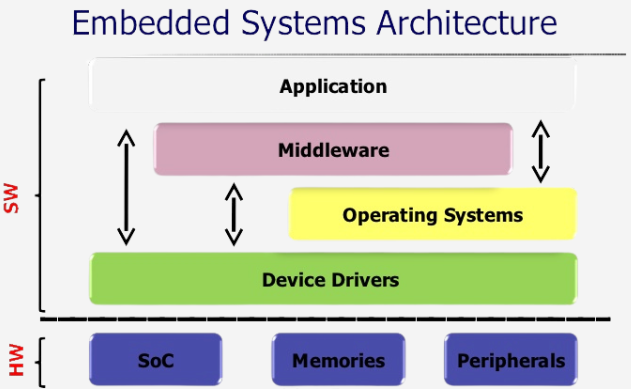
\includegraphics[width=\textwidth]{Pics/embedded_layer_architecture.png}
	\caption{Allgemeine Darstellung der Schichtenarchitektur.\cite{RichardsFord2020}}
	\label{fig:embedded_layer_architecture}
\end{figure}
Die betreffenden Treiber beinhalten Funktionen, welche den Zugriff auf die Hardware mittels sogenannter Register erlauben.
Register sind spezifische Speicherbereiche innerhalb des Microcontrollers, welche eine unmittelbare Manipulation des Hardware-Verhaltens ermöglichen.
Durch das gezielte Setzen oder Auslesen einzelner Bits in diesen Registern ist es möglich, beispielsweise Sensorwerte zu erfassen (z. B. das Drücken eines Tasters) oder Ausgaben zu erzeugen (z. B. das Anzeigen eines Textes auf einem Display).
% Memory Mapped IO
Der Zugriff auf diese Register erfolgt typischerweise über den Mechanismus des \gls{mmio}. 
In diesem Prozess werden die Peripherieregister in denselben Adressraum eingebunden wie der Arbeitsspeicher (RAM). 
Für den Prozessor ist es somit irrelevant, ob er Daten im RAM oder in einem Peripherieregister liest oder schreibt – beide Zugriffe erfolgen über die gleichen Speicherbefehle. 
Der wesentliche Unterschied zwischen den beiden Verfahren liegt darin, dass ein Zugriff auf ein Register nicht nur die Daten verändert, sondern auch das Verhalten der Hardware steuert oder deren aktuellen Status zurückgibt.
\gls{mmio} zeichnet sich zum einen durch die direkte Hardwaresteuerung aus.
Jeder Registerzugriff löst eine konkrete Aktion aus.
Ein Nachteil besteht in den Nebenwirkungen, die beispielsweise das automatische Löschen von Statusbits beim Lesen mit sich bringen.
% Caching und Spekulationsmechanismen
Ein weiteres Problem ist das fehlende Caching, da Peripheriebereiche von Cache- und Spekulationsmechanismen ausgeschlossen werden müssen. 
Diese Peripheriebereiche liegen im \gls{mmio} Bereich.
Damit dürfen diese nicht über einen Cache gelesen oder beschrieben werden, da der Prozessor sonst mit veralteten oder falschen Werten arbeiten oder Schreibzugriffe nicht korrekt bei der Hardware ankommen würden.
Darüber hinaus setzen moderne Prozessoren häufig sogenannte Spekulationsmechanismen ein, bei denen Befehle vorab ausgeführt werden, um die Leistung zu steigern.
Im Falle eines spekulativen Zugriffs einer CPU auf Speicherzugriffe im MMIO-Bereich besteht die Möglichkeit einer ungewollten Veränderung der Registerzustände, beispielsweise durch das vorzeitige Löschen von Statusbits.
Um derartige Seiteneffekte zu unterbinden, werden Speicherbereiche für Peripherie explizit als \texttt{device memory} oder \texttt{strongly ordered} markiert, sodass spekulative Zugriffe auf diese Bereiche unterbunden werden.
% Keyword: volatile
Zudem besteht die Notwendigkeit, in höheren Programmiersprachen wie C oder C++ Registerzugriffe als \texttt{volatile} zu deklarieren, um unzulässige Compileroptimierungen zu verhindern.
Das Schlüsselwort \texttt{volatile} weist den Compiler explizit darauf hin, dass der Wert einer Variablen oder eines Speicherbereichs sich jederzeit außerhalb der Programmlogik ändern kann. Ein Beispiel für eine solche Änderung sind Hardwareereignisse oder Interrupts.
Dadurch wird verhindert, dass Lese- oder Schreibzugriffe wegoptimiert, zwischengespeichert oder in ihrer Reihenfolge verändert werden.
Insbesondere bei Zugriffen auf Speicherbereiche im Kontext von \gls{mmio} ist dies von essenzieller Bedeutung, da jeder Zugriff direkt mit der Hardware interagiert und somit zwingend ausgeführt werden muss, um den korrekten Zustand der Peripherie sicherzustellen.


\subsection{Microcontroller Unit (MCU)}
Ein Microcontroller ist ein vollständig auf einem einzigen Chip realisierter Mikrocomputer, der neben dem eigentlichen Prozessor (CPU) auch sämtliche für den Betrieb notwendigen Komponenten integriert. 
Zu den Komponenten eines solchen Systems zählen in der Regel Programmspeicher (Flash), Datenspeicher (\gls{ram}), digitale Ein- und Ausgänge (\gls{gpio}), Timer, Kommunikationsschnittstellen (wie \gls{uart}, \gls{spi}, \gls{i2c}, \gls{can}) sowie in vielen Fällen analoge Peripheriekomponenten wie Analog/Digital-Wandler oder Pulsweitenmodulation-Einheiten.

Microcontroller werden für spezifische Steuerungs- und Regelungsaufgaben konzipiert und finden typischerweise Anwendung in eingebetteten Systemen, wie beispielsweise Haushaltsgeräten, Fahrzeugsteuerungen, Industrieanlagen oder IoT-Geräten. 
Die Geräte zeichnen sich durch einen geringen Energieverbrauch, eine kompakte Bauform, niedrige Kosten und eine direkte Hardwareansteuerung aus. 
Im Vergleich zu Mikroprozessoren sind für den Grundbetrieb von Microcontrollern keine externen Komponenten erforderlich, was besonders kompakte und zuverlässige Systemlösungen ermöglicht.


\subsection{Peripherie}
Unter dem Begriff der \emph{Peripherie} versteht man im Kontext der Embedded-Softwareentwicklung sämtliche Ein- und Ausgabeschnittstellen, die eine Interaktion des Microcontrollers mit seiner Umwelt ermöglichen.
Peripheriegeräte stellen die Verbindung zwischen der digitalen Rechenlogik des Microcontrollers und der realen Welt her.
Sie ermöglichen die Erfassung, Verarbeitung und Ausgabe physikalischer Signale wie Temperatur, Licht oder der Betätigung eines Tasters.
Ein moderner Microcontroller, wie etwa ein STM32, ist bereits mit einer Vielzahl an integrierten Peripherieeinheiten ausgestattet, darunter digitale Ein-/Ausgänge (GPIOs), serielle Kommunikationsschnittstellen (UART, SPI, I2C, CAN), analoge Wandler (ADC, DAC), Timer oder PWM-Module (Pulsweitenmodulation). 
Die als \emph{On-Chip} bezeichneten Komponenten sind integraler Bestandteil des Microcontrollers und können über zugehörige Register programmiert und gesteuert werden.
Zusätzlich zur integrierten Peripherie besteht die Möglichkeit, über die physischen Pins des Microcontrollers auch externe Peripheriegeräte anzuschließen. 
Die Verbindung erfolgt in der Regel mittels Steckverbindungen, wie etwa Jumper-Kabeln, Steckbrücken, Pin-Headern oder speziellen Anschlussleisten auf Entwicklungsboards. 
In der Regel werden zu diesem Zweck Steckbretter (Breadboards) oder Lochrasterplatinen verwendet, um eine übersichtliche und flexible Verdrahtung zu gewährleisten. 
Externe Bauteile, wie etwa Sensoren (Temperatursensor), Aktoren (LED), Displays oder Speicherbausteine, werden über gängige Schnittstellen wie I2C, SPI, UART oder digitale GPIOs mit dem Microcontroller verbunden.
Die Kommunikation mit externen Geräten wird durch die Peripheriemodule des Microcontrollers realisiert. 
Für den zuverlässigen Betrieb sind in der Regel spezifische Softwaretreiber erforderlich, die die Initialisierung, Datenübertragung und gegebenenfalls die Fehlerbehandlung übernehmen.

\subsubsection*{General Purpose Input Output}
Der Begriff "General Purpose Input/Output" (GPIO) bezeichnet universelle, digitale Pins eines Microcontrollers, die flexibel als Eingang oder Ausgang konfiguriert werden können.
Sie stellen die grundlegendste Form der Interaktion mit der Außenwelt dar und gestatten die Erfassung externer digitaler Signale, z.B. von Tastern oder Sensoren, sowie die Erzeugung entsprechender Signale etwa zur Steuerung von LEDs oder Relais.
Grundsätzlich können GPIOs flexibel als Eingang oder Ausgang verwendet werden.
Typischerweise erfolgt die Konfiguration solcher Embedded-Systeme statisch während der Initialisierung, entweder automatisch durch Codegeneratoren wie STM32CubeMX oder manuell in der Startkonfiguration der Firmware.
Obwohl eine Änderung der GPIO-Funktionalität zur Laufzeit technisch möglich wäre, wird dies in der Praxis häufig vermieden, um ein deterministisches und stabiles Systemverhalten zu gewährleisten.
In der praktischen Anwendung bilden sie die Grundlage für einfache Steuerungs- und Überwachungsaufgaben und sind daher von zentraler Bedeutung für die hardwarenahe Embedded-Programmierung.

\subsubsection*{Serial Peripheral Interface}
Die Schnittstellen des \emph{Serial Peripheral Interface} (SPI) ist ein synchrones, serielles Kommunikationsprotokoll, das insbesondere für die schnelle und effiziente Datenübertragung über kurze Distanz zwischen einem Master- und einem oder mehreren Slave-Geräten eingesetzt wird. 
Die primäre Aufgabe des Protokolls besteht in der Verbindung von \gls{mcu}s mit integrierten oder externen Komponenten, zu denen unteranderem  Sensoren, Speicher, Aktoren sowie Displays zählen.
SPI arbeitet synchron, d.h. Sender und Empfänger teilen sich ein gemeinsames Taktsignal.
Der Master ist derjenige, der diesen Takt vorgibt und bereitgestellt.
Dadurch wird eine präzise, zeit-sensitive Übertragung ermöglicht. 
Die zentrale Eigenschaft von \gls{spi}, die das gleichzeitige Senden und Empfangen ermöglicht ist die Unterstützung der Voll-Duplex-Kommunikation.
% TODO: SPI: Quellenverweise einfügen.
Der \gls{spi}-Bus verwendet meistens vier physikalische Leitungen:
\begin{itemize}
	\item \gls{mosi} / \gls{copi} für die Kommunikation vom Master zu den Peripheriegeräten (Slaves).
	\item \gls{miso} / \gls{cipo} für die Kommunikation von den Peripheriegeräten zum Master.
	\item \gls{ss} / \gls{cs} für die Auswahl des gewünschten Peripheriegerätes.
	\item \gls{sclk} als Taktleitung, die den vom Master vorgegebenen Takt enthält.
\end{itemize}

In der Regel dient der Microcontroller als Master, der den Datenfluss steuert.
Mittels des Slave-Signals ist es der \gls{mcu} möglich, gezielt Slaves anzusprechen.
Dabei ist darauf zu achten, dass jeweils nur ein Slave die Kommunikation aktiv durchführen darf, um eine Kollision auf Bus zu vermeiden.

\gls{spi} zeichnet sich im Vergleich zu anderen seriellen Protokollen wie \gls{i2c} durch eine vereinfachte Implementierung und eine deutlich höhere Datenübertragungsrate aus. 
Allerdings fehlen eine standardisierte Adressierung und Fehlerprüfung, was den Einsatz auf kurze Distanzen und überschaubare Topologien begrenzt. 

%\subsubsection*{Controller Area Network}
%Das \emph{Controller Area Network} (CAN) ist ein robustes, serielles, asynchrones Bussystem, das insbesondere in der Automobilindustrie eine weite Verbreitung findet. 
%Es ermöglicht eine zuverlässige Kommunikation zwischen mehreren Steuergeräten (Nodes), auch unter schwierigen elektromagnetischen Bedingungen. 
%Der Einsatz von CAN in sicherheitskritischen Anwendungen beruht auf zwei wesentlichen Eigenschaften: 
%\begin{itemize}
%	\item der prioritätsbasierten Arbitrierung
%	\item der integrierten Fehlererkennung
%\end{itemize}
% 
%Diese Eigenschaften gewährleisten eine hohe Ausfallsicherheit.
%Die CAN-Technologie basiert auf einem \emph{shared medium} mit Bus-Topologie, bei der alle Teilnehmer über zwei Leitungen mit einander verbunden sind.
%Jede im CAN-Bus übertragene Nachricht ist durch eine eindeutige Identifikationsnummer gekennzeichnet, die sich auf die Art der übertragenen Information bezieht, beispielsweise Geschwindigkeit, Drehzahl oder Sensordaten. 
%Für jede Identifikationsnummer ist ausschließlich ein Knoten zur Übertragung von Nachrichten mit dieser Kennung vorgesehen, um Konflikte im Bus zu vermeiden. 
%Alle angeschlossenen Knoten sind prinzipiell in der Lage, diese Nachrichten zu empfangen, müssen dies jedoch nicht zwingend tun. 
%Jeder Knoten entscheidet autonom, welche Nachrichten für ihn relevant sind, und verarbeitet ausschließlich diese. 
%Ein Absender oder Empfänger ist in der Nachricht selbst nicht kodiert, sodass die Kommunikation vollständig nachrichtenbasiert und nicht adressbasiert erfolgt.
%Es ist grundsätzlich möglich, dass mehrere Knoten auf dieselbe Nachricht reagieren.
%
%Ein wesentliches Merkmal ist die prioritätsbasierte Arbitrierung. 
%Jeder Knoten hat die Möglichkeit, eine Nachricht gleichzeitig zu senden. 
%Das Protokoll verwendet ein bitweises Arbitrierungsverfahren. 
%Nachrichten mit einer niedrigeren ID (höhere Priorität) durchdringen das System automatisch, ohne dass es zu Kollisionen oder Datenverlust kommt.
%Dieses Verfahren zeichnet sich durch seine besondere Effizienz aus und ist in der Lage, Echtzeitanforderungen zu erfüllen.
%
%Obwohl CAN asynchron arbeitet, d.h. jeder Knoten verfügt über einen eigenen Takt, erfolgt die Synchronisation der Kommunikation durch ein fein abgestimmtes Zeitraster innerhalb des CAN-Controllers. 
%Die Bitzeit wird in sogenannte Zeitquanten (Time Quanta, TQ) unterteilt, deren Definition relativ zur eingestellten Bus-Baudrate erfolgt. 
%Diese Zeitquanten lassen sich in mehrere Segmente unterteilen: 
%
%\begin{itemize}
%	\item Synchronisationssegment, das der Flankenerkennung dient, 
%	\item das Propagationssegment, das die Signallaufzeiten berücksichtigt,
%	\item die Segmente für die Phase 1 und Phase 2, die für die Feinjustierung des Abtastzeitpunkts verantwortlich sind.
%\end{itemize}
%
%Der Sample Point ist definiert als der Zeitpunkt, an dem der Wert des Bits für alle Knoten einheitlich abgetastet wird. 
%Dieser befindet sich zwischen Phase 1 und Phase 2. 
%Die interne Taktfrequenz der CPU beeinflusst dabei lediglich die Genauigkeit der Generierung der Zeitquanten, während die tatsächliche Bitdauer durch die konfigurierte \emph{Baudrate} des CAN-Busses bestimmt wird.
%

\section{Software}

\label{sec:architecture_design_pattern}
\subsection{Architektur- und Designmuster}

\begin{figure}[H]
	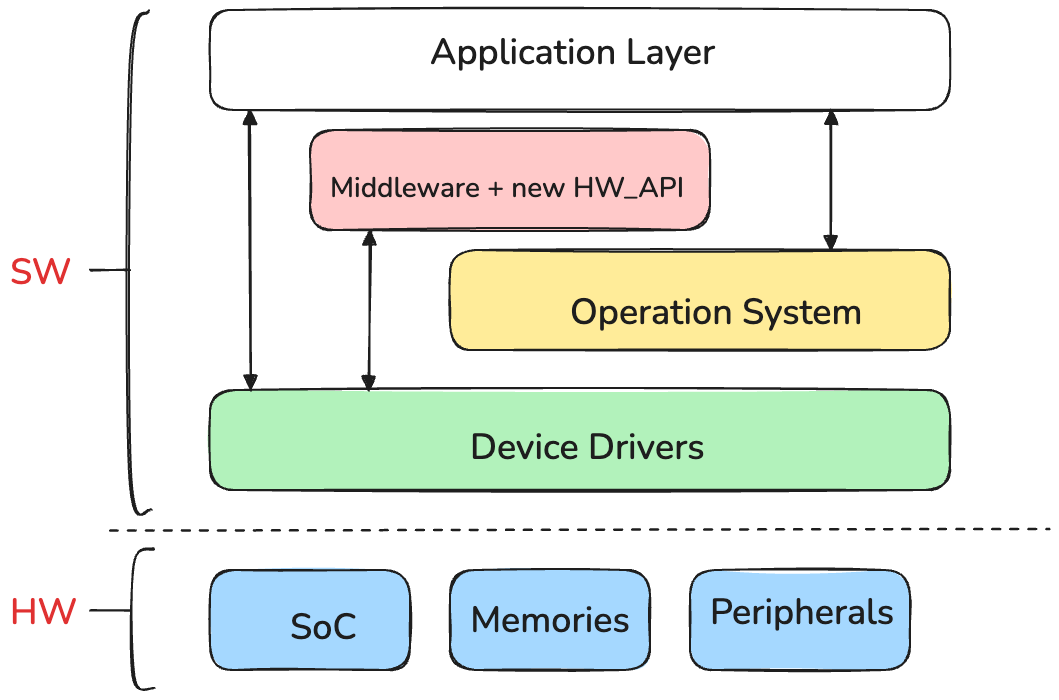
\includegraphics[width=\textwidth]{Pics/layer_architecture_hw_api.png}
	\caption{Darstellung der Schichtenarchitektur inklusive der neuen Hardware-API.}
	\label{fig:layer_architecture_hw_api}
\end{figure}

\subsubsection{Architekturmuster}
%Unter Architektur, speziell \emph{Softwarearchitektur} versteht man den Prozess eine allgemeine Struktur für ein Softwaresystem zu erstellen.
Helmut Balzert definiert den Begriff als ''eine strukturierte oder hierarchische Anordnung der Systemkomponenten sowie Beschreibung ihrer Beziehungen'' \cite{balzert2011softwaretechnik2}.
In diesem Prozess gilt es, die Komponenten in eine grobe (high-level) Gliederung zu bringen.
Im Kontext der Embedded Systeme und Entwicklung und speziell dieser Arbeit, wird sich primär mit der \emph{Schichtenarchitektur} befasst.

Bei diesem Architekturmuster wird das gesamte System in Schichten unterteilt, die  Handlungsbereiche darstellen.
Diese Schichten funktionieren so, dass sie nur mit der direkt anliegenden tieferen Schicht kommunizieren können.
Das bedeutet eine Schicht $n$ kann nur mit der Schicht $n-1$ kommunizieren und ist von dieser abhängig.
Schicht $n-1$ bietet dabei die entsprechenden Funktionen für Schicht $n$.
Umgekehrt gilt diese Abhängigkeit aber nicht.

Im Embedded Bereich lassen sich die Schichten wie folgt beschreiben:

\paragraph{Anwendungsschicht/Application Layer}
dient als oberste Schicht.
Diese besteht aus allen Dateien, Funktionen und Klassen, die nicht direkt mit den auf Hardwareebene liegenden Registern zu tun haben; so z.B. Hilfsfunktionen.
Stattdessen werden die Funktionen der nächst tieferen Schicht verwendet.

\paragraph{Mittelschicht/Middleware}
als optionale zweite Schicht, befasst sich mit möglichen Zusatzfunktionen wie USB, Netzwerkanschlüsse (WLAN), Bluetooth oder IoT (Internet of Things) oder \gls{api}-Funktionen.
Sie dient als verteilende Zwischenschicht zwischen der Programm und der Abstraktionsschicht der Hardware.
\cref{fig:layer_architecture_hw_api} zeigt, wo die neu entwickelte Hardware-API in den Bereich der Middleware platziert sein wird.


\paragraph{Betriebssystem} ist eine weitere optionale Schicht.
Optional in dem Sinn, das ein Embedded System nicht zwingend eine Betriebssystem benötigt.
Dann wird von Bare-Metal-Entwicklung gesprochen.
Ohne das Betriebssystem werden direkt die Pins, d.h. die Hardware angesprochen und programmiert; z.B. wenn in kleinem Schaltkreis nur ein Schalter, mit dem ein Signal ein oder ausgeschalten werden soll, und eine LED, die mit dem Schaltersignal leuchtet oder nicht, verbaut sind.
Das Programm befindet sich dann in einem sog. \textit{Superloop}, einer endlosen Schleife, in der alle Aufgaben des Systems sequentiell und wiederholt abgearbeitet werden, ohne dass ein Betriebssystem zur Ablaufsteuerung oder Taskverwaltung erforderlich ist.
Wird ein Betriebssystem eingesetzt bringt das funktionale Erweiterungen mit sich, wie Multitasking oder besseres Zeitmanagement.
Des weiteren muss bei mit einem OS (Operating System) auf die verfügbaren Ressourcen geachtet werden, da der Speicher bei Microcontrollern begrenzt ist.

\paragraph{Hardwareabstraktionsschicht} (\gls{hal}) befindet sich unter der Middleware bzw. unter dem Betriebssystem.
Gibt es keine zusätzlichen Funktionen in der Middlewareschicht und wird bare-metal entwickelt kann aus der Applikation direkt auf die hier gelagerten Funktionen zugreifen.
Wie dieser direkte Zugriff auf die Abstraktionsschicht aussieht ist in Code \cref{lst:stm32_mx_gpio_init}
zu sehen.
\clearpage

\begin{lstlisting}[language=C, caption={Funktion zur Initialisierung der GPIO-Pins aus einem STM32-Projekt.}, label={lst:stm32_mx_gpio_init}]
int main(void)
{
  HAL_Init();
  SystemClock_Config();
  MX_GPIO_Init();
  
  while (1){ ... } 
}

static void MX_GPIO_Init(void)
{
  GPIO_InitTypeDef GPIO_InitStruct = {0};

  /* GPIO Ports Clock Enable */
  __HAL_RCC_GPIOC_CLK_ENABLE();
  __HAL_RCC_GPIOF_CLK_ENABLE();
  __HAL_RCC_GPIOA_CLK_ENABLE();

  /*Configure GPIO pin Output Level */
  HAL_GPIO_WritePin(LEDextern_GPIO_Port, LEDextern_Pin, GPIO_PIN_RESET);

  /*Configure GPIO pin : LEDextern_Pin */
  GPIO_InitStruct.Pin = LEDextern_Pin;
  GPIO_InitStruct.Mode = GPIO_MODE_OUTPUT_PP;
  GPIO_InitStruct.Pull = GPIO_NOPULL;
  GPIO_InitStruct.Speed = GPIO_SPEED_FREQ_LOW;
  HAL_GPIO_Init(LEDextern_GPIO_Port, &GPIO_InitStruct);
}
\end{lstlisting}

Aus der \texttt{int main(void)}, der Hauptfunktion wird die Funktion \texttt{static MX\_GPIO\_Init(void)} zur Initialisierung der Pins aufgerufen.

In dieser Funktion wird erst eine Struktur \texttt{GPIO\_InitStruct} vom Typ \texttt{GPIO\_InitTypeDef} vorbereitet, indem alle Werte, die in der Struktur enthalten sind gleich $0$ gesetzt werden.
Danach werden für die verwendeten Ports die jeweiligen Clocks gestartet, damit jeder Port auch eine Takt hat;
gefolgt von dem Zurücksetzen des GPIO-Pins, damit dieser keine ungewünschten Werte ausgibt, die evtl. zuvor in dem Register standen.
Mit \texttt{ HAL\_GPIO\_WritePin(LEDextern\_GPIO\_Port, LEDextern\_Pin, GPIO\_PIN\_RESET);} wird sichergestellt, dass der Pin auf $0$ gesetzt ist.
Ab jetzt wird die vorbereitete Struktur mit Werten belegt.
Damit die Funktion \texttt{HAL\_GPIO\_Init()} weiss, welchen Pin sie initialisieren muss, bekommt die Struktur die einzelnen Eigenschaften des Pins übergeben.
So bestimmt 
\begin{itemize}
	\item \texttt{GPIO\_InitStruct.Pin} um welchen Pin es sich handelt, 
	\item \texttt{GPIO\_InitStruct.Mode} in welchem Modus der Pin operieren soll,
	\item \texttt{GPIO\_InitStruct.Pull} welche Art von internem Widerstande (Pull-Up, Pull-Down oder kein Pullwiderstand) verwendet werden soll,
	\item \texttt{GPIO\_InitStruct.Speed} mit welcher Schaltgeschwindigkeit der Pin arbeitet, d.h. wie schnell ein Flankenwechsel erfolgen darf und welche Anstiegszeit für die Signale zugelassen wird.
\end{itemize}

Am Ende dieser Funktion sieht man \texttt{HAL\_GPIO\_Init(GPIO\_Port, \&GPIO\_InitStruct)}.
Diese Funktion ist Teil der Hardwareabstraktionsschicht, auf die hier ohne weitere Zwischenschicht oder Betriebssystem zugegriffen wird.

\paragraph{Die Treiberschicht} 
ist die letzte Ebene vor der Hardwareschicht.
Diese Schicht arbeitet eng mit der Abstraktionsschicht zusammen.
Sie enthält neben den Low-Level-Treibern, die direkten Zugriff auf die Register haben, den in Assembler geschriebenen Startupcode und Initialisierungsroutinen.


\subsubsection{Designmuster} \label{chap3_2_1_designmuster}
% TODO: Designpattern: Nur für OOP?
Neben dem Architekturmuster, das für die Struktur des gesamten Projekts verantwortlich ist, stehen die \emph{Designmuster}.
Unter diesem Begriff versteht man das Designen von einzelnen Softwarekomponenten, wie diese aufgebaut sein sollen, wie sie miteinander kommunizieren, welche Eigenschaften sie haben und hilft dabei die Software zu implementieren.
Designmuster konzentrieren sich somit auf das Innenleben eines Projekts.\cite{gfg_DesignVsArchitecture}

Dabei wird unterschieden zwischen
\begin{itemize}
	\item \textbf{Erzeugungsmuster},
	\item \textbf{Strukturmuster} und
	\item \textbf{Verhaltensmuster}.
\end{itemize}

Erzeugungsmuster helfen dabei, die Art und Weise der Erzeugung von Objekten umzusetzen.
Sie sorgen dafür, dass der eigentliche Erzeugungsprozess nicht direkt sichtbar.
Der Fokus liegt auf der Trennung von der Erzeugung und Verwendung von Objekten, um Flexibilität, Wiederverwendbarkeit und Austauschbarkeit zu ermöglichen.
Beispiel, die im Laufe dieser Arbeit noch erscheinen sind das Factory-Pattern, das Singleton-Pattern oder das Builder-Pattern.
%% Factory
Das Factory-Pattern dient der Kapselung des Erzeugungsprozesses, indem die Instanziierung von Objekten an eine spezielle Fabrikklasse oder -methode ausgelagert wird. 
Es ist nicht erforderlich, dass dem aufrufenden Code der konkrete Typ des zurückgegebenen Objekts bekannt ist. 
Dies hat eine erhöhte Austauschbarkeit und Erweiterbarkeit zur Folge.

%% Singleton
Das sogenannte Singleton-Pattern stellt sicher, dass von einer bestimmten Klasse lediglich eine Instanz existiert und diese global zugänglich ist. 
Typischerweise findet es Anwendung, um zentrale Ressourcen wie Konfigurationsobjekte oder Schnittstellen konsistent bereitzustellen.

%% Builder
Das Builder-Pattern dient der schrittweisen und flexiblen Erzeugung komplexer Objekte.
Dabei werden die Eigenschaften dieser Objekte nacheinander gesetzt. 
Auf diese Weise wird eine klare Trennung zwischen dem Erstellungsprozess und der finalen Darstellung erreicht.

Strukturmuster helfen dabei, die erstellten Klassen und Objekte zu organisieren.
Der Fokus liegt auf dem Zusammenspiel unabhängig entwickelter Klassenbibliotheken sowie der Vereinfachung von Schnittstellen und dem modularen Aufbau von Systemen.
%% Facade
Das sogenannte Facade-Pattern dabei stellt eine Methode dar, um eine einheitliche und vereinfachte Schnittstelle zu einem komplexen Subsystem bereitzustellen. 
Dies hat den Vorteil, dass Implementierungsdetails verborgen werden und die Verwendung der Schnittstelle für den Anwender erheblich vereinfacht wird.

Verhaltensmuster definieren, wie Objekte miteinander interagieren, wie Zuständigkeiten aufgeteilt werden und wie der Kontrollfluss zwischen ihnen abläuft.
Der Fokus liegt nicht ausschließlich auf dem ''Was'' (z. B. ein Event), sondern auch auf dem ''Wie'', ''Wann'' und ''Wer''.
Ein Beispiel hierfür ist die Template Method. 
In Muster definiert eine Basisklasse einen Algorithmus, d.h. eine feststehende Reihenfolge von Befehlen oder Funktionen. 
Die Implementierung aller Schritte wird dabei nicht durch die Basisklasse selbst vorgenommen, sondern kann für die jeweiligen einzelnen Zwischenschritte, sogenannter Hooks, individuell durch Unterklassen erfolgen.
Im Rahmen der STM32-HAL wird dieses Muster bei Callback-Funktionen für Interrupts verwendet. 
Die Funktion \texttt{HAL\_GPIO\_EXTI\_IRQHandler(uint16\_t GPIO\_Pin)} fungiert als Template, während die Funktion \texttt{HAL\_GPIO\_EXTI\_Callback(uint16\_t GPIO\_Pin)} als Hook vom Entwickler selbst implementiert werden muss.

\subsection{Application Programming Interface}
Eine \emph{Anwendungsprogrammierschnittstelle} (\gls{api}) wird von IBM beschrieben ''eine Reihe von Regeln oder Protokollen, die es Softwareanwendungen ermöglichen, miteinander zu kommunizieren, um Daten, Funktionen und Funktionalitäten auszutauschen.''\cite{ibmAPI}.
Damit soll eine Vereinfachung und Effizienzsteigerung für die Softwareentwicklung erreicht werden.
\glspl{api} dienen als Zwischenschicht zwischen verschiedenen Softwarekomponenten oder Systemen.
Sie ermöglichen eine klare Abgrenzung der Zuständigkeiten und stellen eine Abstraktion komplexer interner Abläufe hinter einer standardisierten Schnittstelle bereit.
So können beispielsweise Anwendungen Datenformate automatisch anpassen oder Funktionen anderer Programme nutzen, ohne deren interne Implementierung kennen zu müssen.
Eine solche standardisierte Schnittstelle ermöglicht es die \gls{api}-Funktionen wieder zu verwenden, so dass Entwickler diese nicht immer wieder neu implementieren müssen.
Gleichzeitig wird zur allgemeinen Sicherheit beigetragen, da nur definierte Informationen nach außen weitergegeben werden und der Zugriff von außen gezielt eingeschränkt.

%Dies hat zur Folge, dass Geräte oder Server ihre Daten nicht vollständig aufdecken müssen.

\subsection{CMake}
CMake ist ein plattformübergreifendes Open-Source-Werkzeug zur Automatisierung des Buildprozesses in der Softwareentwicklung
Der sogenannte Metabuild-Generator (\autoref{fig:cmake_generators}) dient als eine Art universeller Konfigurator, der mithilfe Konfigurationsdateien, den \texttt{CMakeLists.txt}-Dateien, spezifische Build-Systeme für eine Vielzahl unterschiedlicher Plattformen und Entwicklungsumgebungen generiert.
Unter diesen Build-Systemen finden sich beispielsweise Makefiles für Unix/Linux, Projektdateien für Visual Studio oder Xcode.

\begin{figure}[H]
	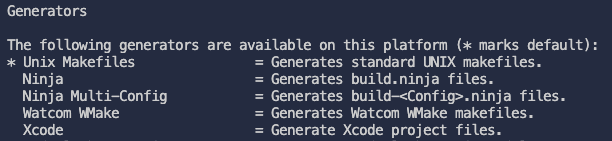
\includegraphics[width=\textwidth]{cmake_generators.png}
	\caption{Ausschnitt einer Liste von verfügbaren Generatoren.}
	\label{fig:cmake_generators}
\end{figure}

Ein wesentlicher Vorteil von CMake liegt in der Trennung von Quell- und Build-Verzeichnissen, was sogenannte Out-of-Source-Builds ermöglicht.
Diese Vorgehensweise trägt zur Schaffung einer übersichtlichen Projektstruktur bei und vereinfacht die Verwaltung von Build-Artefakten.
Zusätlich fördert CMake die hierarchische Strukturierung von Projekten mittels der Implementierung von modularen CMakeLists.txt-Dateien in Unterverzeichnissen.
Dieser Ansatz steigert die Wartbarkeit und Skalierbarkeit komplexer Softwareprojekte.

\subsection{Make und Makefiles}
Make ist ein traditionelles Werkzeug zur Automatisierung von Build-Prozessen, das sogenannte Makefiles zur Steuerung dieser Prozesse einsetzt.
Die Makefiles definieren Regeln, mit deren Hilfe der Quellcode, abhängig davon ob sich etwas im Code geändert hat, kompiliert und verlinkt wird.
Make findet für gewöhnlich Anwendung in der direkten Steuerung von Kompilierungsprozessen.
 Es besteht jedoch auch die Möglichkeit, es zur Steuerung anderer Build-Systeme einzusetzen.
In einigen Projekten findet ein manuelles Makefile Verwendung, welches ausschließlich CMake mit spezifischen Parametern aufruft, um den eigentlichen Build-Prozess zu initialisieren.
In einem solchen Szenario fungiert Make als Wrapper über CMake und ersetzt nicht dessen eigentliche Build-Logik.

































\chapter{Stand der Technik}
In diesem Kapitel erfolgt eine Untersuchung des aktuellen Stands der Technik im Bereich der hardwarenahen Softwareentwicklung für Mikrocontroller.
Das Ziel besteht darin, bestehende Ansätze und Konzepte zu analysieren, die das Problem der Treiberauswahl und -abstraktion lösen – insbesondere im Hinblick auf Portabilität und Wiederverwendbarkeit. 
In der vorliegenden Untersuchung wird eine Analyse der gegenwärtig in der Praxis und Forschung eingesetzten Methoden vorgenommen. 
Ziel dieser Analyse ist es, die Übereinstimmung dieser Ansätze mit den Anforderungen der jeweiligen Zielsetzung zu ermitteln und deren Eignung für die Umsetzung einer eigenen Lösung zu evaluieren.

Die Analyse dient zudem der Identifikation möglicher Lücken oder Einschränkungen bestehender Lösungen und trägt somit zur Begründung der Relevanz und Zielsetzung dieser Arbeit bei.


\section{Recherche}
Im Rahmen der Untersuchung wurden sowohl wissenschaftliche Publikationen als auch praxisnahe Quellen herangezogen. 
Zu den praxisnahen Quellen zählen technische Dokumentationen, Open-Source-Projekte und Herstellerdokumentationen.
Der Fokus der Recherche lag auf bestehenden Lösungen für die plattformübergreifende Auswahl von Hardwaretreibern für Mikrocontroller.
Die im Rahmen der Untersuchung verwendeten relevanten Schlüsselbegriffe umfassten unter anderem \textit{Hardware Abstraction Layer, Embedded Driver Portability, CMSIS, Arduino Core, Zephyr RTOS,C++ Hardware API Design}.

Auf diese Weise wurden verschiedene Ansätze zur Hardwareabstraktion und Treiberbereitstellung gefunden.
Die \emph{Common Microcontroller Software Interface Standard} (CMSIS)-Bibliothek ist eine von ARM entwickelte Schnittstelle, die eine weit verbreitete Anwendung findet. 
Sie bietet eine einheitliche Zugriffsebene für Cortex-M-Prozessoren. 
Herstellerbezogene Entwicklungsumgebungen wie die STM32CubeIDE von STMicroelectronics und die Espressif-IDE bieten umfangreiche Hardware-Abstraktionsbibliotheken, die gezielt auf ihre jeweiligen Mikrocontroller-Familien zugeschnitten sind.

Darüber hinaus wurden zwei Open-Source-Projekte auf GitHub analysiert: mcu-cpp und modm. 
Die Zielsetzung beider Ansätze besteht in der Modularisierung der Treiberentwicklung in C++ sowie der Bereitstellung portabler, wiederverwendbarer Hardware-APIs. 
Die Projekte zeigen eine Reihe unterschiedlicher Herangehensweisen in Bezug auf Abstraktionslevel, Architektur und Hardwareunterstützung, was wertvolle Erkenntnisse für die eigene Lösungsentwicklung bietet.
\\
\\
In den folgenden Absätzen werden die einzelnen Plattformen bewertet und potentiellen Vor- und Nachteile benannt; auch in Bezug auf die Anforderungen der eigenen Lösung. 
%Wie machen das andere; auch in Form kommerzieller Werkzeuge (cubeIDE, Espressif):
%\begin{itemize}
% 	\item CMSIS
%	\item Espressif IDE
%\end{itemize}

\section{Bewertung der Alternativlösungen}
\subsection{STM32Cube}
Die STM32Cube-Umgebung der Firma STMicroelectronics bietet ein gesamtes System, von der Auswahl und der Konfiguration der Hardware bis hin zu einer IDE zur Softwareentwicklung und einer Software um den internen Speicher der MCUs zu programmieren.
Aufgeteilt auf:
\paragraph{STMCUFinder}
	um die Hardware zu finden, die den notwendigen Anforderungen gerecht werden kann.
	Dafür gibt es die Möglichkeit, mit verschiedenen Filtern die Auswahl derart einzuschränken, dass nur noch die passenden Mikrokontroller übrig bleiben.
	Diesen Schritt kann man nicht nur allein für die MCUs und MPUs machen, sondern auch für gesamte Hardwareboards.
	Hier kommen Filter hinzu, welche Funktionen die Hardware bereits integriert hat.
	Ist die passende Hardware ausgewählt, kann aus dieser Übersicht direkt der STM32CubeMX gestartet werden.

\paragraph{STM32CubeMX} 
	zur Konfiguration der Hardware, d.h. Benennung und Funktionszuweisung der Pins, Aktivieren oder Deaktivieren von Registern und Protokollen, Konfiguration der internen Frequenzen. 
	Nach der Konfiguration kann der Code für das Projekt generiert werden.
	In diesem Schritt werden die notwendigen Pakete, Treiber (HAL, CMSIS) und Firmware für die ausgewählte Hardware geladen.

\paragraph{STM32CubeIDE}
	um Anwendungen und Software für die MCUs zu entwickeln und implementieren.
	Die Entwicklungsumgebung, basierend auf Eclipse, bietet neben dem Codeeditor ein eigenes Buildsystem, das mit Make und der \texttt{arm-none-ebai-gcc}-Toolchain arbeitet und einen Debugger hat, mit dem nicht nur Code sondern auch das Verhalten der Hardware beobachtet werden kann um Fehler zu erkennen.
\\
\\
Hier ist Positiv hervorzuheben, dass sehr viel über eine Benutzeroberfläche eingerichtet werden kann, was den Einstieg in die Embedded-Entwicklung etwas leichter gestaltet.
Durch das große Portfolio an an MCUs und Hardwareboards, die alle mit der STM32Cube-Umgebung kompatibel sind, ist es nicht direkt notwendig andere Optionen in betracht zu ziehen. 
Allerdings ist das auch ein Aspekt, der bedacht werden muss. 
Das Softwarepaket funktioniert nur mit der STM32-Hardware.
Der Einsatz mit MCUs anderer Hersteller ist damit nicht vorgesehen.

Für allgemeine Projekte bzw. st-fremde Hardware besteht die Möglichkeit, in der STM32CubeIDE leere CMake-Projekte zu erstellen.
Hier müssen dann die benötigten Pakete und Treiber selber inkludiert werden.
Ein Buildsystem müsste selber eingebunden und mit eigenen CMake-Dateien implementiert werden.


% TODO: chap4 Espressif-IDE
%\subsection{Espressif-IDE}

% TODO: chap4 mcu-cpp & modm: Tiefer Analyse: Wie ist der Code aufgebaut -> Architektur-Muster

\subsection{mcu-cpp}
% TODO: chap4 mcu-cpp: Quellen-Verlinkung
Das Open-Source-Projekt \emph{mcu-cpp} verwendet einen eigenen \texttt{namespace} um die einzelnen Funktionen und Klassen zu gruppieren.
\emph{Namespaces} sind eine Möglichkeit in C++ um Variablen, Klasse und Funktionen zu gruppieren, damit Konflikte bei der Benennung solcher Identifizierer zu vermeiden.
Die ermöglicht einen sauber-strukturierten und lesbaren Applikationscode zu schreiben, in dem man nachvollziehen kann, wer was aufruft.
Basierend auf den virtuellen Klassen, implementieren die jeweiligen MCUs die Methoden damit diese für sich funktionieren.
Um innerhalb einer Produktfamilie, z.B. STM32F0 MCUs, die richtigen bzw. alle notwendigen Ports zu aktivieren, gibt es eine zusätzliche Datei \texttt{gpio\_hw\_mapping.hpp}.
In dieser werden einzelne Ports, die nicht auf jeder MCU verfügbar sind, durch bedingte Kompilierung aktiviert oder nicht.
Die Information, welche Hardware verwendet wird, muss entweder in der \texttt{CMakeLists.txt} oder im Code mit \texttt{\#define} angegeben sein.
Zusätzlich werden die CMSIS-Treiber verwendet, die die Startdateien bereit stellen.
Als RTOS wird aktuell FreeRTOS verwendet.
%Dies ermöglicht
Allerdings fehlen hier die offizielle \emph{Hardware-Abstracition-Layer} (HAL), die bereits vorgefertigte Strukturen und Funktionen für die einzeln Hardwarefunktionen implementiert haben.
Stattdessen werden diese durch die Implementierung der virtuellen Klassen ersetzt.
Das sorgt im weiteren Verlauf dafür, dass die Funktionen auf Basis der virtuellen Klassen für jede neue MCU-Familie neu implementiert werden muss, was einen für wiederholten Aufwand sorgt und den Anforderungen an die Lösung widerspricht.



\subsection{modm}
% TODO: chap4 modm: Quellen-Verlinkungß
Das Open-Source-Projekt \emph{modm} dient als Baukasten um zugeschnittene und anpassbare Bibliotheken für Mikrocontroller zu generieren.
Dadurch ist es möglich, dass eine Bibliothek nur aus den Teilen besteht, die tatsächlich in der Applikation und im Code verwendet werden müssen, ohne das es einen unnötig großen Overhead gibt.
Um das zu bewerkstelligen wird eine Kombination aus \texttt{Jinja2}-Template-Dateien, \texttt{lbuild}-Pyhton-Skripte und eigenen Moduldefinitionen verwendet, mit der der Code für die Bibliotheken generiert wird.
Die Templatedateien enthalten Platzhalter.
Die Werte kommen aus \texttt{YAML} und \texttt{JSON}-Dateien, die von den \texttt{lbuild}-Pyhtonskripten gelesen und in die entsprechenden Positionen der Platzhalter, während des Buildprozesses, eingefügt werden.
 
Um eine Bibliothek zu erstellen, muss ein Prozess über die Konsole gestartet werden.
modm hat bereits vordefinierten Konfigurationen für eine große Auswahl an MCUs.
Mit diesen kann die Bibliothek für ein Projekt erstellt/gebuildet werden.

Will man aber Module verwenden, die in der vordefinierten Konfiguration nicht enthalt sind, kann man Module einzeln zu der \texttt{project.xml} hinzufügen.
Um sehen zu können welche Module zur Verfügung stehen muss folgende Zeile in der Konsole ausgeführt werden:

\vspace{3mm}
\begin{lstlisting}[language=bash, caption={Konsolenbefehl um verf\"ugbare Module aufgelistet zu bekommen; hier f\"ur den STM32C031C6T6 Mikrokontroller.}, label={lst:modm_lbild_discover}]
\modm\app\project>
	lbuild --option modm:target=stm32c031c6t6 discover
\end{lstlisting}

Sobald die gewünschten Module hinzugefügt wurde, beginnt der Installations- bzw. der Generierungsprozess der Library. 
Gibt man nun \texttt{lbuild builld} in der Konsole ein wenn man sich im \texttt{app/project}-Verzeichnis kann die Bibliothek erstellt werden.
Nach erfolgreichem Build erscheint in dem Projektverzeichnis ein neuer Ordner \emph{modm}.
Dieser enthält die generierten Dateien der ausgewählten Module.

Positiv hervorzuheben ist hier das (vordergründige) simple Hinzufügen von Modulen.
Da das Projekt aktuell bereits sehr umfangreich ist und sehr viele Mikrokontroller und Optionen unterstützt, bietet es eine große Auswahl an Modulen, die beliebig zu einem Projekt hinzugefügt werden können.

Allerdings ist zu beachten, dass falls man zukünftig neue Module oder Mikrokontroller hinzufügen will, müssen diese an die bestehende Struktur angepasst und in das Zusammenspiel von Python, Jinja2 und den YAML/JSON-Dateien integriert werden.
Dies ist mit einem sehr hohen Aufwand verbunden.


%%%%%%%%%%%%%%%%%%%%%%%%%%%%%%%%%%%%%%%%%%%%%%%%%%%%%%%%%%%%%%%%%%%%
% Notizen
%%%%%%%%%%%%%%%%%%%%%%%%%%%%%%%%%%%%%%%%%%%%%%%%%%%%%%%%%%%%%%%%%%%%
\section{Notizen}
Ähnlich zu dem Projekt mcu-cpp soll die eigene Lösung auch Interfaces bzw. virtuelle Klassen als Basis verwenden, die dann von allen MCUs abstrahiert werden können.
Auf diese Weise bekommt jede MCU eine eigene Kindklasse, über die die richtigen Treiber ausgewählt werden.



\begin{itemize}
	\item Interface/virtuelle Klassen als Basis
	\item \textbf{Factory Methode} zur Erzeugung der Objekte $\rightarrow$ Entwurf der Architektur
	\item [$\Rightarrow$] Adapter implementieren um andere MCUs verwenden.
	\item [$\Rightarrow$] Was muss alles bedacht werden:
	\begin{itemize}
		\item Pin Initialisierung $\rightarrow$ STM32 ok; wie bei anderen MCUs?
		\item Interrupt-Handling
		\item 
		\item Flashen des Chips mit dem Programm
	\end{itemize}
	\item einfache Make commands rufen CMake build commands auf
	\item Ninja als Generator $\rightarrow$ wird von ESP, mcu-cpp, Zephyr schon benutzt. STM32 nutzt make, kann aber getauscht/angepasst/konfiguriert werden
	\item Treiber (HAL, vllt. CMSIS) als Submodule
\end{itemize}

\subsection{Architektur}
\subsubsection*{Factory}
\begin{itemize}
	\item erstellt und returned Hardware-Instanz
	\item für HW-Inistialisierung
	\item erstellt Instanz je nach Hardware $\rightarrow$ \texttt{\#ifdef}
\end{itemize}

\subsubsection*{Peripherie: GPIO, SPI, UART}
\begin{itemize}
	\item eigene Klasse
	\item erstmal für STM32 $\rightarrow$ danach Adapter für andere?
\end{itemize}

Keine \texttt{setter}
\begin{itemize}
	\item Pin wird nur einmal initialisiert
	\item normalerweise keine nachträgliche Änderungen zur Laufzeit
\end{itemize}

%%%%%%%%%%%%%%%%%%%%%%%%%%%%%%%%%%%%%%%%%%%%%%%%%%%%%%%%%%%%%%%%%%%%
% PROBLEME
%%%%%%%%%%%%%%%%%%%%%%%%%%%%%%%%%%%%%%%%%%%%%%%%%%%%%%%%%%%%%%%%%%%%
\subsection*{Probleme:}
\begin{itemize}
	\item Interruptfunktionen $\rightarrow$ werden automatische aufgerufen und nicht vom Entwickler. Wenn ein Interrupt auftritt wird der Rest der HAL \& der MCU informiert.\\ \textbf{Frage:} Wie kann es umgesetzt werden, dass das GPIO-Objekt der API und der Code der Anwendungsschicht aus der HAL und den Registern über einen Interrupt informiert werden?
	\item \texttt{\_\_HAL\_RCC\_GPIOA\_CLK\_ENABLE()} setzt den Pin im Inputregister IDR $\rightarrow$ ID14.
	
\end{itemize}

\subsection*{Gelöst}
\begin{itemize}
	\item GPIO init $\rightarrow$ MX\_GPIO\_Init() startet mit \texttt{iocurrent} bei $0$. Mit dem Aufruf durch das Objekt startet \texttt{iocurrent} auf etwas extrem Hohen. \\ $\Longrightarrow$ Ist Egal. \texttt{iocurrent} bekommt direkt einen richtigen Startwert zugewiesen.
	\item Statt \texttt{ID15} für Pin 15 zu wechseln, werden die \texttt{ID0-3} gewechselt. Diese ersten $4$ Pin ergeben binär auch $15\ =\ 1111\ =\ 1*2^3\ +\ 1*2^2\ +\ 1*2^1\ +\ 1*2^0$ \\ \textbf{Lösung:} Nicht den Wert $15$ dem Pin Attribut geben sondern am Bit $15$, dass diese Bit dann auf $1$ gesetzt wird.
	\item Wenn die LED an ist, d.h. wenn der Pin gesetzt ist, verändert sich der Pin des Tasters, ohne dass dieser betätigt wurde. Wieso?\\ \textbf{Beobachtung:} Ob bei \texttt{readPin()} Register ID$14$ oder ID$9$ verwendet wird (es sollte $9$ sein; $14$ ist nur im Debugger aktiv und für uns uninteressant) schon zufällig zu sein.\\ \textbf{Lösung:} Mit Pin-Debouncing und Implementierung einer Timer-Klasse konnte das zufällige Verhalten gelöst werden. 
	\item Mit \texttt{time.hpp} und \texttt{stm32::Gpio::Pull::Up} funktioniert die Schaltung.\\ \textbf{Frage:} Wieso funktioniert das mit \texttt{Pull::Up} und nicht mit \texttt{Pull::None} od. \texttt{Pull::Down}?\\ \textbf{Antwort:} Mit \texttt{Pull::None} befindet sich der Schalter in einem \emph{float} Zustand. In diesem werden besonders Einflüsse der Umwelt, sog. Noise/Rauschen aufgenommen, die das Verhalten der Schaltung unberechenbar machen. Dieses zufällige Verhalten sollte vermieden werden, besonders in einem sicherheitskritischen Umfeld.
\end{itemize}

\vspace{3mm}

mapping $\rightarrow$ stm32c0xx.h $\rightarrow$ stm32c031xx.h mit allen TypeDefs $\rightarrow$ system\_stm32c031xx.h

$\Longrightarrow$ include Fehler: statt nur stm32\_hal\_gpio.h, besser stm32\_hal.h einbinden.
\\

Verwendung von STM32CubeIDE für bessere Übersicht beim Debuggen über die Register.
\\

%\vspace{3mm}
%\begin{figure}[H]
%	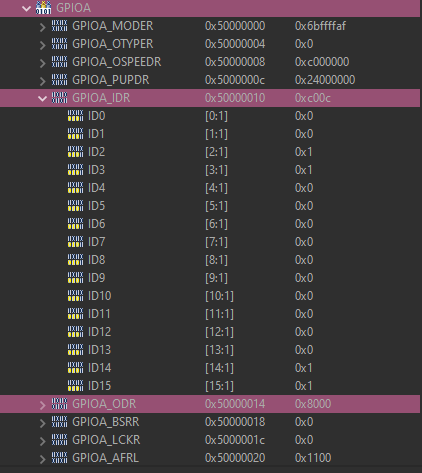
\includegraphics[width=\textwidth]{stm32_c031c6_clean_registers_setPin.PNG}
%	\caption{Register beim setzen des Pin.}
%	\label{fig:stm32_register_setPin}
%\end{figure}
%
%\vspace{3mm}
%\begin{figure}[H]
%	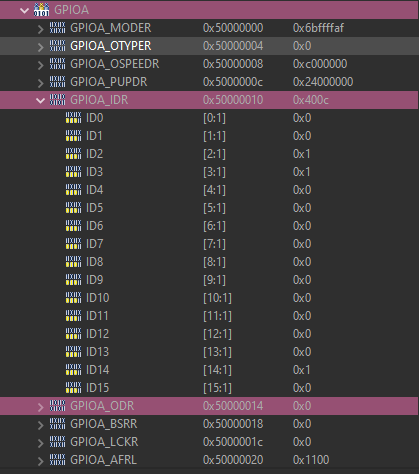
\includegraphics[width=\textwidth]{stm32_c031c6_clean_registers_resetPin.PNG}
%	\caption{Register beim zurücksetzen des Pin.}
%	\label{fig:stm32_register_resetPin}
%\end{figure}
%
%In den Abbildungen \autoref{fig:stm32_register_setPin} und \autoref{fig:stm32_register_resetPin} ist der Wert von Pin 15 (ID15 \& OD15) zu beobachten. Bei \texttt{0x0} wird der Pin zurückgesetzt und die LED leuchtet nicht mehr. Bei \texttt{0x1} wird der Wert auf $1$ gesetzt und die LED beginnt zu leuchten.
%
%Die Funktionen \texttt{HAL\_GPIO\_WritePin(GPIO\_TypeDef \*GPIOx, uint16\_t GPIO\_Pin, GPIO\_PinState PinState)} steuern nicht die in \autoref{fig:stm32_register_setPin} und \autoref{fig:stm32_register_resetPin} gezeigten Register IDR und ODR an, sondern die Set- und Reset-Register BSRR und BRR. 
%
%Diese Register sind \emph{write only}, d.h. sie können nicht ausgelesen werden.
%Wird die Funktion korrekt ausgeführt, kann dass Verhalten an den Registern IDR und ODR beobachtet werden.






























\chapter{Konzeption der API}
In diesem Teil der Arbeit wird ein Konzept der API erstellt.
Das Wissen, das durch die vorherigen Kapitel erlangt wurde, hilft dabei zu erkennen, welchen Aspekten besondere Beachtung gegeben werden muss.
Der Aufbau dieses Konzepts passiert in mehreren Schritten:
\begin{itemize}
	\item [1.]  Anforderungsanalyse: \\In diesem Abschnitt werden die wichtigen Eigenschaften, die die API haben muss zusammengetragen. Daneben wird analysiert, wie die Funktionen, die enthalten sein sollen aufgebaut und implementiert werden können. Dafür werden die notwendigen, existierenden Funktionen der jeweiligen \gls{hal} (STM32 und ESP32) auf etwaige Gemeinsamkeiten untersucht.
 	\item [2.] 	Betrachtung bestehender Lösungen: \\Mit den zusammengetragenen Eigenschaften werden bereits existierende Lösungen und deren Ansätze betrachtet. Hierbei stehen  neben der STM32CubeIDE und der ESP-IDF speziell zwei Projekte im Fokus: \href{https://github.com/yh-sb/mcu-cpp.git}{mcu-cpp}\cite{github_mcu_cpp} und \href{https://github.com/modm-io/modm.git}{modm}\cite{github_modm}
	\item [3.] Architekturentwurf: \\Hier werden passende Architekturmuster für das gesamte System der API und Designmuster für mögliche Module evaluiert; welches Muster erfüllt die erarbeiteten Eigenschaften am besten.
	\item [4.] Implementierung: \\Anhand der erstellten Softwarearchitektur wird ein Testprojekt erstellt, das die einzelnen Module implementiert. Um die korrekte Funktionsweise des Codes zu verifizieren, wird die in Abschnitt \ref{chap2_rahmenbedingungen} genannte Hardware verwendet. 
\end{itemize}




\chapter{Durchführung}
\section{Anforderungsanalyse}
Um eine benutzerfreundlichen und leistungsfähigen API-Bibliothek entwickeln zu können, ist es wichtig die grundlegenden Funktionen klar zu definieren.
So gilt es als erstes die Fragen zu klären: \emph{Was muss die API können?} und \emph{Welche Eigenschaften soll die API haben?}\\
% Allgemeines Ziel; Pin-Objekte
Es ist das übergeordnete Ziel, plattformunabhängigen Code schreiben zu können.
Das bedeutet, es muss möglich sein ein Programm, das z.B. für eine Hardware mit einem STM32-\gls{mcu} geschrieben wurde, auch für Hardware mit einer ESP32-\gls{mcu} funktionsfähig zu haben.
Die spezifische Konfiguration der Hardware und der Pins, wie sie beispielsweise mit STM32CubeMX gemacht werden kann, muss dennoch für jede Hardware, je nach Projekt, neu erstellt werden.
Dies liegt unter anderem an den unterschiedlichen Prozessorarchitekturen, der Anzahl an Pins und deren Zuordnung zu spezifischen Funktionen oder der Registerkonfiguration.
Um eine Pinkonfiguration mit Code zu lösen und von der graphischen Oberfläche wegzukommen, liegt der Gedanke nahe, Objekte zu verwenden.
Besonders im Kontext der Verwendung von C++.
Solche Objekt werden mittels eines Konstruktors, der die Werte für die Attribute der Pins übergeben bekommt, erstellt.
Bevor eine Erstellung dieser Pin-Objekte stattfinden kann, Aufgrund der angesprochen Unterschiede, muss erst die Hardware ausgewählt werden.
% Hardware- und Treiberauswahl
Damit die Pin-Objekte auch verwendet werden können, muss vorher die Hardware ausgewählt und initialisiert werden.
Beginnend mit der Auswahl, muss die API in der Lage sein, nach einer Art der Definition, welche Hardware real zur Verfügung steht, die passenden Treiber auszuwählen, eine Instanz der Hardware zu erstellen, mit der im Programm gearbeitet werden kann und aus diesem heraus die Hardware über allgemein definierte Funktionen mit den richtigen Treibern zu initialisieren.
Diese Definition kann beispielsweise über ein \texttt{\#define}, dass den Namen der Hardware beinhaltet gelöst werden.
Mit Blick auf zukünftige Veränderungen sollte es auch so einfach wie möglich sein, weitere Hardware der API hinzu zu fügen, um die Auswahl zu erweitern.
Diese Veränderungen und Erweiterungen würden auch die jeweiligen Peripheriefunktionen betreffen.
Um einen klaren Überblick über diese Funktionen zu behalten, ist der Gedanke an Module zu betrachten.
So könnte für jede Peripheriefunktion (\gls{gpio}, \gls{spi}, \gls{uart}, \gls{can}) ein eigenes Modul implementiert werden.
Auf diese Weise hat man neben dem Überblick auch eine klare Struktur, die Fehlersuchen und Wartungen der Software wiederum vereinfacht.
% Peripheriemodule
Die Peripheriemodule müssen ähnlich der Hardwareauswahl, die Funktionen der Hardware kapseln.
Im Fall der STM32-\gls{mcu}s werden die Funktionen der eigenen \gls{hal}-Bibliothek verwendet.
ESP32 Hardware hat hierbei seine eigene \gls{hal} mit zugeschnittenen Funktionen.



\section{Betrachtung bestehender Lösungen}
In diesem Abschnitt erfolgt eine Untersuchung des aktuellen Stands der Technik im Bereich der hardwarenahen Softwareentwicklung für Microcontroller.
Das Ziel besteht darin, gemeinsame Eigenschaften heraus zu arbeiten, verwendete Architekturmuster zu identifizieren und bestehende Ansätze und Konzepte zu analysieren, die das Problem der Treiberauswahl und -abstraktion lösen – insbesondere im Hinblick auf Portabilität und Wiederverwendbarkeit. 

Die Analyse dient zudem der Identifikation möglicher Lücken oder Einschränkungen bestehender Lösungen und trägt somit zur Begründung der Relevanz und Zielsetzung dieser Arbeit bei.

Im Rahmen der Untersuchung wurden neben Onlinerecherchen speziell praxisnahe Quellen herangezogen. 
Zu diesen zählen technische Dokumentationen, Open-Source-Projekte und Herstellerdokumentationen.
Der Fokus der Recherche lag auf bestehenden Lösungen für die plattformübergreifende Auswahl von Hardwaretreibern für Microcontroller.
Verwendete relevante Schlüsselbegriffe umfassten unter anderem \textit{Hardware Abstraction Layer, Embedded Driver Portability, STM32, ESP32, CMSIS, Arduino Core, Zephyr RTOS,C++ Hardware API Design}.

Auf diese Weise wurden verschiedene Ansätze zur Hardwareabstraktion und Treiberbereitstellung gefunden.
Die Common Microcontroller Software Interface Standard (CMSIS)-Bibliothek ist eine von ARM entwickelte Schnittstelle, die eine weit verbreitete Anwendung findet. 
Sie bietet eine einheitliche Zugriffsebene für Cortex-M-Prozessoren. 
Herstellerbezogene Entwicklungsumgebungen wie die STM32CubeIDE von STMicroelectronics und die Espressif-IDE bieten umfangreiche Hardware-Abstraktionsbibliotheken, die gezielt auf ihre jeweiligen Microcontroller-Familien zugeschnitten sind.

Darüber hinaus wurden zwei Open-Source-Projekte auf GitHub analysiert: mcu-cpp und modm. 
Die Zielsetzung beider Ansätze besteht in der Modularisierung der Treiberentwicklung in C++ sowie der Bereitstellung portabler, wiederverwendbarer Hardware-APIs. 
Die Projekte zeigen eine Reihe unterschiedlicher Herangehensweisen in Bezug auf Abstraktionslevel, Architektur und Hardwareunterstützung, was wertvolle Erkenntnisse für die eigene Lösungsentwicklung bietet.
\\
\\
In den folgenden Absätzen werden die einzelnen Plattformen bewertet und potentiellen Vor- und Nachteile benannt; auch in Bezug auf die Anforderungen der eigenen Lösung. 


\subsection{STM32Cube}
\label{sec:stm32cube}
Das STM32Cube-Ecosystem \cite{stm32cube_ecosystem} der Firma STMicroelectronics bietet ein gesamtes System, von der Auswahl und der Konfiguration der Hardware bis hin zu einer IDE zur Softwareentwicklung und einer Software um den internen Speicher der MCUs zu programmieren.
Die Kernprogramme sind dabei:

\paragraph{STM32CubeMX} 
	dient der Konfiguration der Hardware, d.h. Benennung und Funktionszuweisung der Pins, Aktivieren oder Deaktivieren von Registern und Protokollen, Konfiguration der internen Frequenzen über ein graphische Oberfläche.
	Nach der Konfiguration kann der Code für das Projekt generiert werden.
	In diesem Schritt werden die notwendigen Pakete, Treiber (\gls{hal}, CMSIS % TODO: CMSIS Glossareintrag
	) und Firmware für die ausgewählte Hardware geladen. \cite{stm32cubemx}

\paragraph{STM32CubeIDE}
	dient der Softwareentwicklung für die MCUs zu entwickeln und implementieren.
	Die Entwicklungsumgebung, basierend auf Eclipse, bietet neben dem Codeeditor ein eigenes Buildsystem, das mit Make und der \texttt{arm-none-ebai-gcc}-Toolchain arbeitet und einen Debugger hat, mit dem nicht nur Code sondern auch das Verhalten der Hardware beobachtet werden kann um Fehler zu erkennen. \cite{stm32cubeide}
\\
\\
Wird ein neues Projekt über STM32CubeMX gestartet werden automatisch die benötigten Hardwaretreiber und Firmware heruntergeladen und der Projektstruktur hinzugefügt, gleichzeitig wird ein Coderahmen in C generiert. (Code \ref{lst:stm32_mx_gpio_init} ist Teil dieses generierten Coderahmens.)
%In der Hauptheaderdatei (main.h) befinden sich neben den eingebundenen Headerdateien der Treiber auch die Pindefinitionen, die zuvor konfiguriert wurden.
%In der Hauptprogrammdatei (main.c) sind generierte Funktionen für die Hardwareinitialisierung und die Pininitialisierung zu finden.

Dies Funktioniert im Kosmos der STM32Cube-Plattform sehr gut, allerdings ist dies auch Aspekt der beachtet werden muss:\\
Das Softwarepaket funktioniert nur mit der STM32-Hardware, der Einsatz mit \gls{mcu}s anderer Hersteller ist nicht vorgesehen.
Für allgemeine Projekte bzw. st-fremde Hardware besteht die Möglichkeit, in der STM32CubeIDE leere CMake-Projekte zu erstellen.
Die benötigten Pakete und Treiber, sowie ein Buildsystem müssen dann selber inkludiert und mit eigenen CMake-Dateien implementiert werden.


% Schichtenarchitektur
Untersucht man den Aufbau des gesamten Projekts von der Hauptdatei ausgehend soweit bis die Register in den Funktionen der \gls{hal} erreicht sind, lassen sich Schichten erkennen.
% Anwendungsschicht
Die Anwendungsschicht beinhaltet das Hautprogramm inklusive des Hauptheaders.
% Middleware & RTOS
Ein explizite Middleware und Betriebssystemschicht fehlen in einem blanken Projekt, wenn man diese während des Konfigurationsprozesses nicht explizit hinzugefügt hat.
% CMSIS & HAL
In der Treiber- und Abstraktionsschicht finden sich \gls{hal} und CMSIS-Treiber, mit allen benötigten Funktionen und Definitionen um auf Register zuzugreifen und Pins steuern zu können. 

% Designpattern
Sucht man den Code nach Designmuster lassen sich für alle drei Kategorien Exemplare finden.
Für Erzeugungsmuster lassen sich Vergleiche zu Singleton und Builder finden.
Im Rahmen des Grundlagenkapitels zu Designmuster in \cref{chap3_2_1_designmuster} wurde bereits  ausgeführt, dass mit dem Singleton-Pattern lediglich eine Instanz von einer Klasse existieren darf.
Das Builder-Pattern hingegen beschreibt, wie Objekte aufgebaut werden können.
Anstatt sämtliche Parameter in einem einzigen Aufruf zu übergeben, erfolgt die Konfigurierung sukzessive mittels einer Konfigurationsstruktur, wie beispielsweise der Struktur \texttt{GPIO\_InitStruct}. 
Die vollständige Konfiguration wird erst nach Abschluss des Prozesses mit einem finalen Aufruf initiiert, z. B. findet die eigentliche Initialisierung erst durch die Funktion \texttt{HAL\_GPIO\_Init()}. 
Dies führt zu einer verbesserten Lesbarkeit und Wartbarkeit des Codes und reduziert potenzielle Fehler, die durch inkonsistente Parameterübergaben verursacht werden.
Die \texttt{GPIO\_InitStruct}, die man bereits in \cref{lst:stm32_mx_gpio_init} sehen kann, zeigt Ähnlichkeiten zu dem Builder-Muster.
Die Struktur wird hier ebenfalls Option für Option aufgebaut und erweitert.
Wird \gls{spi} verwendet, kommt eine globale \texttt{SPI\_HandleTypeDef} Instanz dazu, ähnlich dem Singleton-Pattern.
%%% Facade
Bei der Suche nach Strukturmustern lässt sich das Facade-Pattern gut an Code \cref{lst:stm32_mx_gpio_init} erkennen.
Die Funktion \texttt{MX\_GPIO\_Init()} fungiert in diesem Kontext als Fassade, indem sie die komplexe Initialisierung mehrerer GPIOs hinter einem einzigen Funktionsaufruf verschleiert.
Anstatt dass der Entwickler die einzelnen Schritte wie Taktfreigabe, Pin-Reset und Konfiguration mit \texttt{HAL\_GPIO\_Init()} selbst durchführen muss, werden diese Details verborgen und über eine einheitliche Schnittstelle bereitgestellt. 
Diese Vorgehensweise dient der Vereinfachung der Benutzung, ohne dabei die zugrunde liegende Funktionalität zu beeinträchtigen.

Im Bereich Verhaltensmuster findet man die Template Method.
Bei diesem Muster definiert eine Basisklasse ein Algorithmus, d.h. eine feste Reihenfolge von Befehlen oder Funktionen; sie implementiert aber nicht alle Befehle selber.
Einige Zwischenschritte, sog. Hooks, können von Unterklassen implementiert werden.
Im Fall der STM32-\gls{hal} findet man dieses Pattern bei den Callback-Funktionen für Interrupts.
Hier ist der \texttt{void HAL\_GPIO\_EXTI\_IRQHandler(uint316\_t GPIO\_Pin)} das Template, die \texttt{void HAL\_GPIO\_EXTI\_Callback(uint16\_t GPIO\_Pin)} die Hook-Funktion, die vom Entwickler selber implementiert werden kann.

%Zusammenfassend wird sich hier in einer Schichtenarchitektur bewegt.







\subsection{Espressif-IDF}
\label{sec:esp_idf}
Aufbau / Ebenene
\begin{itemize}
	\item main
	\item Funktionen
	\item Funktionen $\rightarrow$ HAL-Funktion
	\item HAL-Funktion $\rightarrow$ LL-Funktion
	\item 
\end{itemize}

Das ESP-IDF (Espressif IoT Development Framework) stellt ein offizielles Entwicklungsframework für die Microcontroller der Firma Espressif dar, wie etwa das ESP32 und dessen Varianten. 
Es stellt ein umfangreiches Ökosystem bereit, das sowohl die Auswahl und Konfiguration der Hardware als auch die Entwicklung, das Flashen und Debugging von Software einschließt.

Anders als bei der STM32Cube-Umgebung gibt es hier ein primär Paket, das für die Entwicklung installiert werden muss.
Im Rahmen dieser Installation werden die erforderlichen Softwarekomponenten automatische mit integriert.
Zu diesen Komponenten zählen:

\paragraph{Toolchain}
bringt passende Compiler und die erforderlichen Werkzeuge zum Übersetzen des Quellcodes für die jeweilige ESP32-Plattform. 
Diese beinhalten die Xtensa GCC Toolchain (\texttt{xtensa-esp32-elf-gcc}) für ältere Modelle wie  ESP32-, ESP32-S2- und ESP32-S3-Modelle.
Für neuere Modelle wie den ESP32-C3 und ESP32-C6, die auf RISC-V basieren, wird die RISC-V GCC Toolchain (\texttt{riscv32-esp-elf-gcc}) verwendet.

\paragraph{Build-Tools} 
bestehen aus \texttt{CMake} und \texttt{Ninja} als Generator. 
CMake übernimmt die Konfiguration und Verwaltung des Projektes sowie die Generierung der entsprechenden Build-Files. 
Ninja sorgt für eine schnelle und effiziente Ausführung des eigentlichen Buildprozesses.

\paragraph{Python Skripte}
übernehmen Aufgaben wie die Verwaltung und Konfiguration der Entwicklungsumgebung, das Bauen von Projekten, das Flashen der Firmware auf die Zielhardware sowie die Automatisierung von häufigen Arbeitsabläufen. 
Diese Skripte verwalten im Hintergrund das Framework, sodass der Entwickler selber wenig bis garnicht mit diesen in Kontakt kommt.
Viele Befehle, wie das Kompilieren oder Hochladen, werden über diese Skripte im IDF-Terminal ausgeführt und erleichtern so die Entwicklung und den Workflow mit ESP-IDF erheblich.

\paragraph{Debug-Tools}
wie beispielsweise \texttt{OpenOCD} werden mit installiert.
Diese Werkzeuge ermöglichen neben dem Flashen der Firmware auf die Zielhardware, auch das Setzen von Breakpoints sowie das Debugging direkt auf dem Microcontroller. 
Sie unterstützen verschiedene Schnittstellen (z.\,B. JTAG oder USB) und lassen sich mit gängigen IDEs und Entwicklungsumgebungen integrieren.


Wird ein neues Projekt mit dem ESP-IDF Framework gestartet, erfolgt die Einrichtung der Projektstruktur und der benötigten Komponenten ebenfalls weitgehend automatisiert.
Die Generierung eines neuen Projekts kann über die Kommandozeile des IDF-Terminal oder entsprechende Assistenten wie der ESP-IDF Erweiterung in VSCode erfolgen.
In diesem Prozess generiert das Framework die zugehörige Ordnerstruktur, den Beispielcode sowie die Konfigurationsdateien.
Die erforderlichen Hardwaretreiber, Bibliotheken und Tools wurden bereits mit der Installation des Frameworks bereitgestellt, sodass ein weiterer Download nicht mehr notwendig ist.


Der grundlegende Aufbau eines Projekts im ESP-IDF ist durch eine hierarchische Struktur gekennzeichnet, bei der die einzelnen Ebenen klar voneinander getrennt sind.
Auf oberster Ebene befindet sich die main-Funktion, die den Einstiegspunkt des Programms darstellt.
Von diesem Punkt aus werden die zentralen Initialisierungen ausgeführt und die Steuerung des weiteren Programmablaufs initiiert.
Aus Main-Funktion erfolgt der Aufruf spezifischer Anwendungsfunktionen.
In der Regel erfolgt der Zugriff auf diese Funktionen durch die Verwendung der sogenannten \gls{hal}-Funktionen (Hardware Abstraction Layer).
Das Framework stellt damit einen standardisierten Zugriff auf die zugrunde liegende Hardware bereit.
Die \gls{hal}-Funktionen selbst basieren wiederum auf Low-Level-(LL)-Funktionen, die den direkten Zugriff auf Register und Peripherie des ESP32 ermöglichen.
Diese Schichtung resultiert in einer klare Abstraktion, da die Anwendung hardwareunabhängig entwickelt werden kann, während der Zugriff auf die Peripherie über wohldefinierte Schnittstellen erfolgt.
Zudem besteht bei Bedarf die Möglichkeit, über die LL-Ebene direkt in die Hardware einzugreifen.
Das mehrstufige Konzept zielt darauf ab, sowohl die Portabilität als auch die Wartbarkeit der Software innerhalb des ESP-IDF-Frameworks zu fördern.












































\subsection{mcu-cpp}
\label{sec:mcu_cpp}
Das Open-Source-Projekt \emph{mcu-cpp} \cite{github_mcu_cpp} verwendet einen eigenen \texttt{namespace} um die einzelnen Funktionen und Klassen zu gruppieren.
\emph{Namespaces} sind eine Möglichkeit in C++ um Variablen, Klassen und Funktionen zu gruppieren, damit Konflikte bei der Benennung solcher Identifizierer vermieden werden.
Dies ermöglicht es einen sauber-strukturierten und lesbaren Applikationscode zu schreiben, in dem man nachvollziehen kann, wer was aufruft.
Basierend auf den virtuellen Klassen, werden die jeweiligen Methoden von den \gls{mcu}s implementiert.
Um innerhalb einer Produktfamilie, z.B. STM32F0 MCUs alle notwendigen Ports zu aktivieren, gibt es eine zusätzliche Datei \texttt{gpio\_hw\_mapping.hpp}.
In dieser werden einzelne Ports, die nicht auf jeder MCU verfügbar sind, durch bedingte Kompilierung aktiviert oder nicht.
Die Information, welche Hardware verwendet wird, muss entweder in der \texttt{CMakeLists.txt} oder im Code mit \texttt{\#define} angegeben sein.
Zusätzlich werden die CMSIS-Treiber verwendet, die die Startdateien bereit stellen.
Als RTOS ist FreeRTOS fest im Projekt integriert.
%Dies ermöglicht
Allerdings fehlen hier die offiziellen \emph{Hardware-Abstracition-Layer} (HAL) Funktionen, die bereits vorgefertigte Strukturen und Funktionen für die einzeln Hardwarefunktionen implementiert haben.
Stattdessen werden diese durch die Implementierung der virtuellen Klassen ersetzt.
Das sorgt im weiteren Verlauf dafür, dass die Funktionen auf Basis der virtuellen Klassen für jede neue MCU-Familie neu implementiert werden müssen, was für wiederholten Aufwand sorgt und den Anforderungen an die Lösung widerspricht.

Untersucht man das Projekt auf Architektur- und Designmuster lassen sich die gleichen Muster identifizieren wie bei den STM32-Projekten.
Es wird in einer Schichtenarchitektur gearbeitet.
Die Aufteilung ist nahezu identisch, mit dem Hauptprogramm in der Anwendungsschicht, der Hardwareabstraktion mit den CMSIS Dateien und neu geschriebenen Abstraktionsfunktionen, statt den klassischen \gls{hal}-Bibliothek.
Mit der Verwendung von FreeRTOS kommt hier die Middleware-Schicht, die sich zwischen der Anwendungsschicht und der Abstraktionsschicht befindet, neu hinzu.
% Design
Designmuster ähneln sich ebenfalls.
Für die Hardwareinitialisierung wird das Singleton verwendet.
Es gibt nur eine globale Instanz der \texttt{systick}-Klasse.
Darüber hinaus gibt es keine erkennbaren Erzeugungsmuster.
Die Auswahl der Hardware findet über die Haupt-\texttt{CMakelists.txt}-Datei statt.

Im Bereich der Strukturmuster lässt sich das Facade-Pattern erkennen.
Beispielsweise dient die Klasse gpio\_stm32f4 der Abstraktion der Initialisierung und Steuerung von GPIOs über Registeroperationen in eine klar strukturierte, objektorientierte Schnittstelle. 
Für Entwickler besteht somit die Möglichkeit, GPIOs einfach per Konstruktor und Methoden wie \texttt{set()}, \texttt{toggle()}, \texttt{mode()} oder \texttt{get()} zu verwenden, ohne sich mit den zugrunde liegenden Bitmanipulationen und der Clock-Konfiguration befassen zu müssen. 

Im Bereich der Verhaltensmuster finden sich mehrere Beispiele:

Das Template Method Pattern findet in der \texttt{systick}-Komponente Anwendung. 
Der Ablauf der Interruptbehandlung ist in der entsprechenden Stelle explizit definiert, ermöglicht jedoch die Integration individueller Erweiterungspunkte (beispielsweise durch überschreibbare oder registrierbare Callbacks wie \texttt{onTick()}). 
Diese Erweiterungspunkte können angepasst werden, ohne dabei den Ablauf der Interruptbehandlung selbst zu modifizieren.

Ein weiteres Verhaltensmuster ist das Observer Pattern, das bei der Behandlung von GPIO-Interrupts zum Einsatz kommt.
Die Anwendung ist in der Lage, über Callbacks oder Eventhandler auf externe Ereignisse zu reagieren, die von der Peripherie ausgelöst und vom ISR (Interrupt Service Routine) weitergeleitet werden. 
Hieraus resultiert ein charakteristisches Beobachterverhältnis zwischen Hardwareereignis und Anwendungslogik.

Darüber hinaus lässt sich ein Strategy-Pattern in der SPI-Implementierung identifizieren, bei dem zur Compile- oder Laufzeit unterschiedliche DMA-Komponenten eingebunden werden können. 
Das Verhalten der Datenübertragung unterliegt einer dynamischen Veränderung durch den Austausch von Komponenten.

% TODO: chap4 mcu-cpp: Quellen-Verlinkung


\subsection{modm}
\label{sec:modm}
% TODO: chap4 modm: Quellen-Verlinkungß
Das Open-Source-Projekt \emph{modm} \cite{github_modm}\cite{modm_io}   dient als Baukasten um zugeschnittene und anpassbare Bibliotheken für Microcontroller zu generieren.
Dadurch ist es möglich, dass eine Bibliothek nur aus den Teilen besteht, die tatsächlich in der Applikation und im Code verwendet werden müssen, ohne das es einen unnötig großen Overhead gibt.
Um das zu bewerkstelligen wird eine Kombination aus \texttt{Jinja2}-Template-Dateien, \texttt{lbuild}-Pyhton-Skripte und eigenen Moduldefinitionen verwendet, mit der der Code für die Bibliotheken generiert wird.
Die Templatedateien enthalten Platzhalter.
Die Werte kommen aus \texttt{YAML} und \texttt{JSON}-Dateien, die von den \texttt{lbuild}-Pyhtonskripten gelesen und in die entsprechenden Positionen der Platzhalter, während des Buildprozesses, eingefügt werden.
 
Um eine Bibliothek zu erstellen, muss ein Prozess über die Konsole gestartet werden.
modm hat bereits vordefinierten Konfigurationen für eine große Auswahl an MCUs.
Mit diesen kann die Bibliothek für ein Projekt erstellt werden.

Will man aber Module verwenden, die in der vordefinierten Konfiguration nicht enthalt sind, kann man diese einzeln zu der \texttt{project.xml} hinzufügen.
Um sehen zu können welche Module zur Verfügung stehen muss folgende Zeile in der Konsole ausgeführt werden:

\vspace{3mm}
\begin{lstlisting}[language=bash, caption={Konsolenbefehl um verf\"ugbare Module aufgelistet zu bekommen; hier f\"ur den STM32C031C6T6 Microcontroller.}, label={lst:modm_lbild_discover}]
\modm\app\project>
	lbuild --option modm:target=stm32c031c6t6 discover
\end{lstlisting}

Sobald die gewünschten Module hinzugefügt wurde, beginnt der Installations- bzw. der Generierungsprozess der Library. 
Gibt man nun \texttt{lbuild builld} in der Konsole ein wenn man sich im \texttt{app/project}-Verzeichnis befindet, kann die Bibliothek erstellt werden.
Nach erfolgreichem Build erscheint in dem Projektverzeichnis ein neuer Ordner \emph{modm}.
Dieser enthält die generierten Dateien der ausgewählten Module.

%Positiv hervorzuheben ist hier das (vordergründige) simple Hinzufügen von Modulen.
%Da das Projekt aktuell bereits sehr umfangreich ist und sehr viele Microcontroller und Optionen unterstützt, bietet es eine große Auswahl an Modulen, die beliebig zu einem Projekt hinzugefügt werden können.
%
%Allerdings ist zu beachten, dass falls man zukünftig neue Module oder Microcontroller hinzufügen will, müssen diese an die bestehende Struktur angepasst und in das Zusammenspiel von Python, Jinja2 und den YAML/JSON-Dateien integriert werden.
%Dies ist mit einem sehr hohen Aufwand verbunden.

% Architektur
Wird ein Projekt erstellt, dass eine generierte modm-Bibliothek verwendet, lassen sich auch hier bereits bekannte Muster, wie die Schichtenarchitektur, erkennen.
Anwendungs- und Middlewareschicht unterscheiden sich im Inhalt nicht von dem bereits bekannten aus mcu-cpp und STM32CubeIDE.
Die Anwendungsschicht enthält weiterhin die Hauptdatei, die Businesslogik und eigene erstellt Klassen, die die Funktionen der tieferliegenden Schichten verwenden.
Die Middlewareschicht ist weiterhin optional.
Wurde im Konfigurationsprozess der Bibliothek keine \gls{rtos} oder keine erweiternden Funktionen wie USB und Netzwerkanbindung ausgewählt, sind diese im Projekt ebenfalls nicht vorhanden.
Unterschiede sind in der Abstraktionsschicht zu finden.
Diese verwendet keine bereits vorhandenen Funktionen oder Bibliotheken wie die STM32-\gls{hal}, sondern wird vollständig durch modm generiert.
Sie besteht u.a. aus der Datei \texttt{board.hpp}, die typsichere GPIO-Definitionen, Peripherieklassen (z.B. für SPI und ADC) sowie Funktionen zur Initialisierung und Konfiguration enthält; ähnlich der \texttt{main.h} eines STM32Cube-Projektes.
Dadurch erfolgt eine Kapselung des direkten Zugriffs auf Hardware sowie die Bereitstellung einer objektorientierten API.
Die unterhalb liegende Hardwareschicht besteht aus templatespezifischen Registerzugriffen. 
Funktionen wie \texttt{GpioA0::setOutput()} ermöglichen den direkten Zugriff auf die Register. 
Der Einsatz dieser Low-Level-Operationen erfolgt ausschließlich über die Abstraktionsschicht.
% Designmuster
Im modm-Projekt findet bewusst auf die Verwendung klassischer Designmuster in ihrer typischen objektorientierten Form, verzichtet. 
Stattdessen werden zahlreiche Funktionalitäten durch statische Metaprogrammierung, Templates und generische Programmierung abgebildet. 
Nichtsdestotrotz lassen sich in der Struktur und Verwendung bestimmter Klassen Parallelen zu bekannten Entwurfsmustern erkennen.
%Erzeugungmuster
Ähnlich dem Singleton-Pattern, kann bei einer Vielzahl von GPIO-Objekten und Board-Komponenten, wie beispielsweise \texttt{Board::LedD13} oder \texttt{Board::PushButton}, ein vergleichbare Aufbau beobachten werden.
So ist es möglich, die betreffenden Elemente über statische Typen eindeutig zu referenzieren. 
Dadurch wird eine einzige, globale Instanz je Pin bereitgestellt.

Die Initialisierung über \texttt{Board::initialize()} oder die vordefinierten Aliase wie \texttt{Board::LedD13} können als eine Art Factory betrachtet werden. 
Dies liegt an einer einheitlichen, zentralisierten Bereitstellung von Komponenten für die Anwendung.
Eine echte Factory-Methode im GoF-Sinn ist jedoch nicht implementiert, da keine polymorphe Objekterzeugung zur Laufzeit stattfindet.

Mit Blick auf Strukturmuster können Ähnlichkeiten zum Composite Muster gezogen werden.
Strukturen wie \texttt{GpioSet<GpioA0, GpioA1, GpioA2>} fungieren hierbei als logische Zusammenfassung mehrerer GPIOs.
Obwohl keine echte rekursive Baumstruktur mit abstrakter Basisklasse, wie sie im klassischen Composite Pattern vorliegt, ähneln solche Klassen diesem Muster insofern, als dass sie gemeinsame Operationen, z. B. \texttt{set()}, \texttt{reset()}, auf eine gesamte Gruppe anwenden. 

Ein Verhaltensmuster wie es zuvor in mcu-cpp und STM32Cube-Projekt vorhanden war, ist hier nicht zu erkennen.

Insgesamt fokussiert sich das modm-Projekt auf eine compilezeit-optimierte Architektur, durch die klassische Entwurfsmuster nur begrenzt bzw. in abgewandelter Form eingesetzt werden.
















































































\section{Architekturentwurf}

\label{sec:architecture_properties}
\subsection{Architektonische Eigenschaften der Treiber-API}
Moderen Softwarelösungen bestehen meist aus vielen, großen Dateien, die untereinander von einander abhängig sind.
Um bei solch großen Projekten den Überblick zu behalten, werden diese Softwarelösungen nach gewissen Eigenschaften erstellt.
Diese \emph{architektonischen Eigenschaften} lassen sich (grob) in drei Teilbereiche unterteilen: Betriebsrelevante, Strukturelle und Bereichsübergreifende \cite{barlik_architektur}, wie in Tabelle~\ref{tab:architektonische_eigenschaften} aufgeführt. % Eigenschaften. 

\begin{table}[H]
	\begin{center}
		\begin{tabular}{ c | c | c }
			\textbf{Betriebsrelevante} & \textbf{Strukturelle} & \textbf{Bereichsübergreifende}\\
			%\midrule
			\hline
			Verfügbarkeit & Erweiterbarkeit & Sicherheit\\
			Performance & Modularität & Rechtliches\\
			Skalierbarkeit & Wartbarkeit & Usability\\
			$\cdots$ & $\cdots$ & $\cdots$\\
		\end{tabular}
		\caption{Teilbereiche architektonischer Eigenschaften}
	    \label{tab:architektonische_eigenschaften}
	\end{center}
\end{table}

Aus diesen Eigenschaften gilt es, die wichtigsten für die Treiber-API zu identifizieren. 
Mit diesem Hintergrund lässt sich ein Struktur für das Projekt bilden.

Die Entwicklung einer plattformunabhängigen, wiederverwendbaren Treiber-API für Micro-controller stellt hohe Anforderungen an die Architektur der Softwarebibliothek.

% Welche (architektonischen) Eigenschaft sind wichtig/sollen umgesetzt werden?
% geringe Redundanz
Das Ziel besteht darin, eine Lösung zu schaffen, die sich durch eine geringe Redundanz auszeichnet. 
Die Konzeption von Klassen und Funktionen sollte derart erfolgen, dass eine erneute Implementierung der Applikation für jede neue Plattform nicht erforderlich ist.
Die Wiederverwendbarkeit zentraler Komponenten führt zu einer Reduktion des Entwicklungsaufwands und einer Erhöhung der Konsistenz im Code.

% Usability - Benutzerfreundlichkeit
Ein weiteres zentrales Anliegen ist die einfache Benutzbarkeit. 
Die API ist so zu gestalten, dass eine effiziente Nutzung gewährleistet ist. 
Dies fördert nicht nur die Effizienz in der Erstellung neuer Applikationen, sondern erleichtert auch langfristig die Wartung und Weiterentwicklung der Software.

% Skalierbarkeit
Im Sinne der Skalierbarkeit wird angestrebt, die Lösung auf möglichst viele Microcontroller-Architekturen und Hardwareplattformen anwendbar zu machen.
Die Vielfalt verfügbarer MCUs erfordert eine abstrahierte und flexibel erweiterbare Struktur, die die Integration neuer Plattformen mit minimalem Aufwand ermöglicht.

% TODO chap6: Eigenschaften: Portabilität, ja - nein?
% Portabilität - nochmal anpassen; OS Bezug passt nicht richtig
%Auch die Portabilität spielt eine wichtige Rolle.
%Die Bibliothek sollte nicht nur hardware-, sondern auch betriebssystemunabhängig konzipiert werden.
%Aus diesem Grund wird bei der Entwicklung der Lösung darauf geachtet, dass diese erst unter Windows, später auch unter Linux und macOS einsetzbar ist.
%Die Installation und Konfiguration der dafür benötigten Werkzeuge wird nachvollziehbar dokumentiert, um den Einstieg für die Nutzer zu erleichtern.

% Erweiterbarkeit
Darüber hinaus ist die Erweiterbarkeit ein wesentliches Architekturprinzip
Der Einsatz von leistungsstärkeren Microcontrollern hängt in der Regel mit einer Erweiterung der Funktionalitäten zusammen, die in die bestehenden Treiber- und API-Strukturen integriert werden müssen.
Daher wird großer Wert auf eine modulare und offen gestaltete Architektur gelegt, die neue Features ohne grundlegende Umbauten aufnehmen kann.

% Modularität
Modularität trägt wesentlich zur Übersichtlichkeit und Wartbarkeit des Systems bei. 
Eine saubere Trennung funktionaler Einheiten ermöglicht eine schnellere Lokalisierung und Behebung von Fehlern, was wiederum die langfristige Pflege und Weiterentwicklung der Software erleichtert.

% (Ressourcen-)Effizienz
Schließlich ist auch die Effizienz ein kritischer Aspekt.
Da Microcontroller in der Regel nur über begrenzte Ressourcen verfügen, ist es essenziell, dass die Bibliothek möglichst kompakt und ressourcenschonend implementiert wird. 
Externe Abhängigkeiten werden bewusst auf ein Minimum reduziert, um Speicherplatz zu sparen und unnötige Komplexität zu vermeiden.

Diese architektonischen Prinzipien bilden die Grundlage für die Konzeption und Umsetzung der in dieser Arbeit vorgestellten Treiber-\gls{api}.


\subsection{Architektur- und Designmuster der Treiber-API}

%\begin{itemize}
%	\item Desgin Patterns $\rightarrow$ Aufbau der einzelnen Klassen
%	\begin{itemize}
%		\item Welche werden sonst eingesetzt; welches eignet sich für diesen Zweck
%		\item Wie sollen die Module der jeweiligen Peripherie aufgebaut sein?
%	\end{itemize}
%	\item HardwareInterface mit allen:
%	\begin{itemize}
%		\item vllt. Core: ClockInit, Delay, GetTick
%		\item Gpio
%		\item SPI
%%		\item UART
%		\item CAN
%	\end{itemize}
%\end{itemize}

- Architektonische Eigenschaften\\
- Welche Grundarchitektur liegt vor?\\
- Welches Architekturmuster eignet sich dafür?\\
- Welche Architektur eignet sich hier für? $\rightarrow$ Aufbau des gesamten Systems\\
Um die Struktur der Treiber-\gls{api} zu erstellen, finden die in \cref{sec:architecture_design_pattern} angesprochenen Architektur- und Designmuster Verwendung.
Da sich in der Embeddedwelt bewegt wird, handelt es bei der Gesamtstruktur um ein Schichtenarchitektur.
Das fertige Projekt wird darin eine eigen Schicht bilden.
Damit fehlen noch die Designmuster.
Dieses müssen so ausgewählt werden, dass die Eigenschaften, die in vorherigem \cref{sec:architecture_properties} erarbeitet wurden, bestmöglich erfüllt werden.\\
- C++ $\rightarrow$ Objekt-orientiert\\
- Factory Architektur zur Erstellung von Objekten\\
- Erstellung von Objekten?\\
Beginnend bei der Auswahl der Hardware. 
Factory-Methode:
Interface ruft Factory auf, die eine Instanz des HW-Objektes zurückgibt.
Mit dieser Instanz wird die Hardware initialisiert.
Ein allgemeines Hardwareinterface kapselt Kernfunktionen der Hardware, die für die Systeminitialisierung und -funktionen relevant sind.


Damit aus diesem Interface in Objekt einer spezifischen Hardware wird, bietet sich eine Fabrik an.
Diese wählt anhand der in einer Konfigurationsdatei definierten Hardware die richtige Kindklasse der Interface-Elternklasse aus.

Facade-Pattern:
Eine hardware spezifischere Kindklasse implementiert die Kernfunktionen der Interfaceklasse, passend auf ihr System und erweitert diese um die Peripheriefunktionen.

- Peripheriefunktionen (GPIO, SPI, etc.) als eigenständigen Klassen\\
- Globales Interface\\
- Auswahl der Funktionen\\
Jede Peripheriefunktion wird genau wie die Hardware über eine Interface-Elternklasse und Hardware-spezifische Kindklassen implementiert.

Mit diesem Konzept entsteht ein Modul für jede Peripherie, z.B. das GPIO-Modul.
Diese Module sind so designed, dass sie den tiefergehenden Code hinter einer Facade verbergen.
Durch die vorher definierte Hardware ändert sich am eigentlichen erstellt Programmcode nichts.
Im Hintergrund werden aber die hardware-spezifischen Treiber und HAL Funktionen ausgewählt.
Der Entwickler bekommt davon in der main.cpp nichts mit.


Die grundlegende Struktur des Systems basiert auf einer **Schichtenarchitektur**, wie sie in der Embedded-Softwareentwicklung häufig Anwendung findet. Diese Architekturform ermöglicht eine klare Trennung zwischen Anwendungslogik, Abstraktionsschichten und hardwarenahen Treibern. Die Schichtung erleichtert nicht nur die Wartung und Erweiterbarkeit, sondern trägt auch wesentlich zur Portabilität bei, da einzelne Schichten unabhängig voneinander angepasst oder ausgetauscht werden können. Das entwickelte Projekt bildet dabei eine eigenständige Schicht innerhalb dieser Gesamtarchitektur, die als Schnittstelle zwischen Hardware und Anwendung dient.

Da die Implementierung in **C++** erfolgt, wird die Architektur durch Prinzipien der **Objektorientierung** geprägt. Die Kapselung von Zuständigkeiten in Klassen sowie die Möglichkeit zur Nutzung von Vererbung und Polymorphie bieten eine geeignete Grundlage, um hardwarenahe Funktionalitäten abstrahiert und erweiterbar bereitzustellen. Diese Eigenschaften schaffen die Voraussetzung, Designmuster gezielt einzusetzen, um die im vorangehenden Abschnitt definierten Architekturziele – insbesondere Modularität, Austauschbarkeit und Erweiterbarkeit – zu erreichen.

Ein zentrales Muster stellt dabei die **Factory-Methode** dar. Dieses Erzeugungsmuster dient der Entkopplung von Objektinstanziierung und -nutzung. Für die Hardwareabstraktion bedeutet dies, dass ein allgemeines **Hardwareinterface** definiert wird, das die notwendigen Basisfunktionen bereitstellt. Die konkrete Auswahl und Instanziierung einer spezifischen Implementierung erfolgt über eine Fabrik, die anhand der in einer Konfiguration hinterlegten Zielplattform das passende Objekt erzeugt. Auf diese Weise wird vermieden, dass anwendungsspezifischer Quellcode an hardwareabhängige Details gebunden ist. Die Factory-Methode trägt somit wesentlich zur Erreichung von Plattformunabhängigkeit und Wiederverwendbarkeit des Anwendungscodes bei.

Ergänzend dazu wird das **Fassade-Muster** eingesetzt. Dieses Strukturmuster dient der Vereinfachung des Zugriffs auf komplexe Subsysteme, indem es eine einheitliche Schnittstelle zur Verfügung stellt. In der hier betrachteten Architektur übernehmen hardwarespezifische Kindklassen die konkrete Implementierung der im Interface definierten Kernfunktionen. Über die Fassade werden diese Implementierungen dem Anwendungsentwickler in abstrahierter Form zugänglich gemacht. Dadurch wird die interne Komplexität der hardwarenahen Treiber verborgen, während nach außen eine homogene und stabile Schnittstelle bereitgestellt wird.

Die Architektur wird durch die Modularisierung der **Peripheriefunktionen** weiter verfeinert. Funktionen wie GPIO, SPI oder UART werden jeweils als eigenständige Module entworfen, die wiederum dem Prinzip von Interface und spezifischer Implementierung folgen. Jedes Modul kapselt die hardwarespezifischen Details hinter einer definierten Abstraktionsschicht. Diese konsequente Trennung gewährleistet, dass Änderungen in der Hardware oder den zugrunde liegenden Treibern keine Anpassungen am Anwendungscode erforderlich machen.

Insgesamt entsteht damit eine Architektur, die auf den Prinzipien von **Schichtenarchitektur**, **Objektorientierung** sowie den Designmustern **Factory-Methode** und **Fassade** basiert. Diese Kombination stellt sicher, dass die Softwareportabilität, Erweiterbarkeit und Wartbarkeit erreicht werden, während gleichzeitig die Komplexität für den Anwendungsentwickler reduziert wird.

%Zusammengefasst liegt der Fokus bei der Entwicklung auf diesen Eigenschaften:
%\begin{itemize}
%	\item Skalierbarkeit
%	\item Modularität
%	\item Erweiterbarkeit
%	\item geringe Redundanz
%	\item Effizienz
%	\item Benutzerfreundlichkeit
%\end{itemize}































\section{Implementierung}
Mit der Implementierung wird bei dem Mechanismus zur Auswahl gestartet.

% Fragen
Wie wird der jeweilige Punkt umgesetzt?

Welche Tools werden benutzt/eignen sich besonders für die Umsetzung?
Welche Tools eignen sich für welchen Arbeitsschritt?

Warum wird etwas gerade auf diese Weise umgesetzt?







\section{Validierung}

- Fragen/Anforderungen vom Anfang erfüllt?\\

- Funktionsweise gegeben?\\
- Gpio Test mit Schaltung\\
- Spi Kommunitkation. Test mit Oszi (Screenshots)\\


Die Validierung der entwickelten Hardware-Abstraktionsschicht (HW\_API) dient dem Nachweis ihrer Funktionalität, Korrektheit und Plattformunabhängigkeit. 
Ziel dieser Untersuchung ist es, sicherzustellen, dass die implementierten Klassen sowohl auf STM32- als auch auf ESP32-Plattformen zuverlässig arbeiten und den gestellten Anforderungen entsprechen.
Die Überprüfung der Funktionalität wurden mehreren Schritten gewährleistet.
So musste zunächst bestätigt werden, dass der Code fehlerfrei kompiliert und gebaut wird.
Beim Debuggen musste festgestellt werden, ob das Programm sich so verhält, wie es erwartet ist oder ob unerwünschte Seiteneffekte auftreten.

\subsection{Testaufbau}
Um die korrekte Funktionsweise der Gpio-Klasse zu gewährleisten wurde mit einem Breadboard eine Schaltung mit einem Taster und einer LED aufgebaut.
Diese konnte dann die verfügbaren \gls{mcu}s an den konfigurierten Pins angeschlossen werden.

%\begin{figure}[H]
%	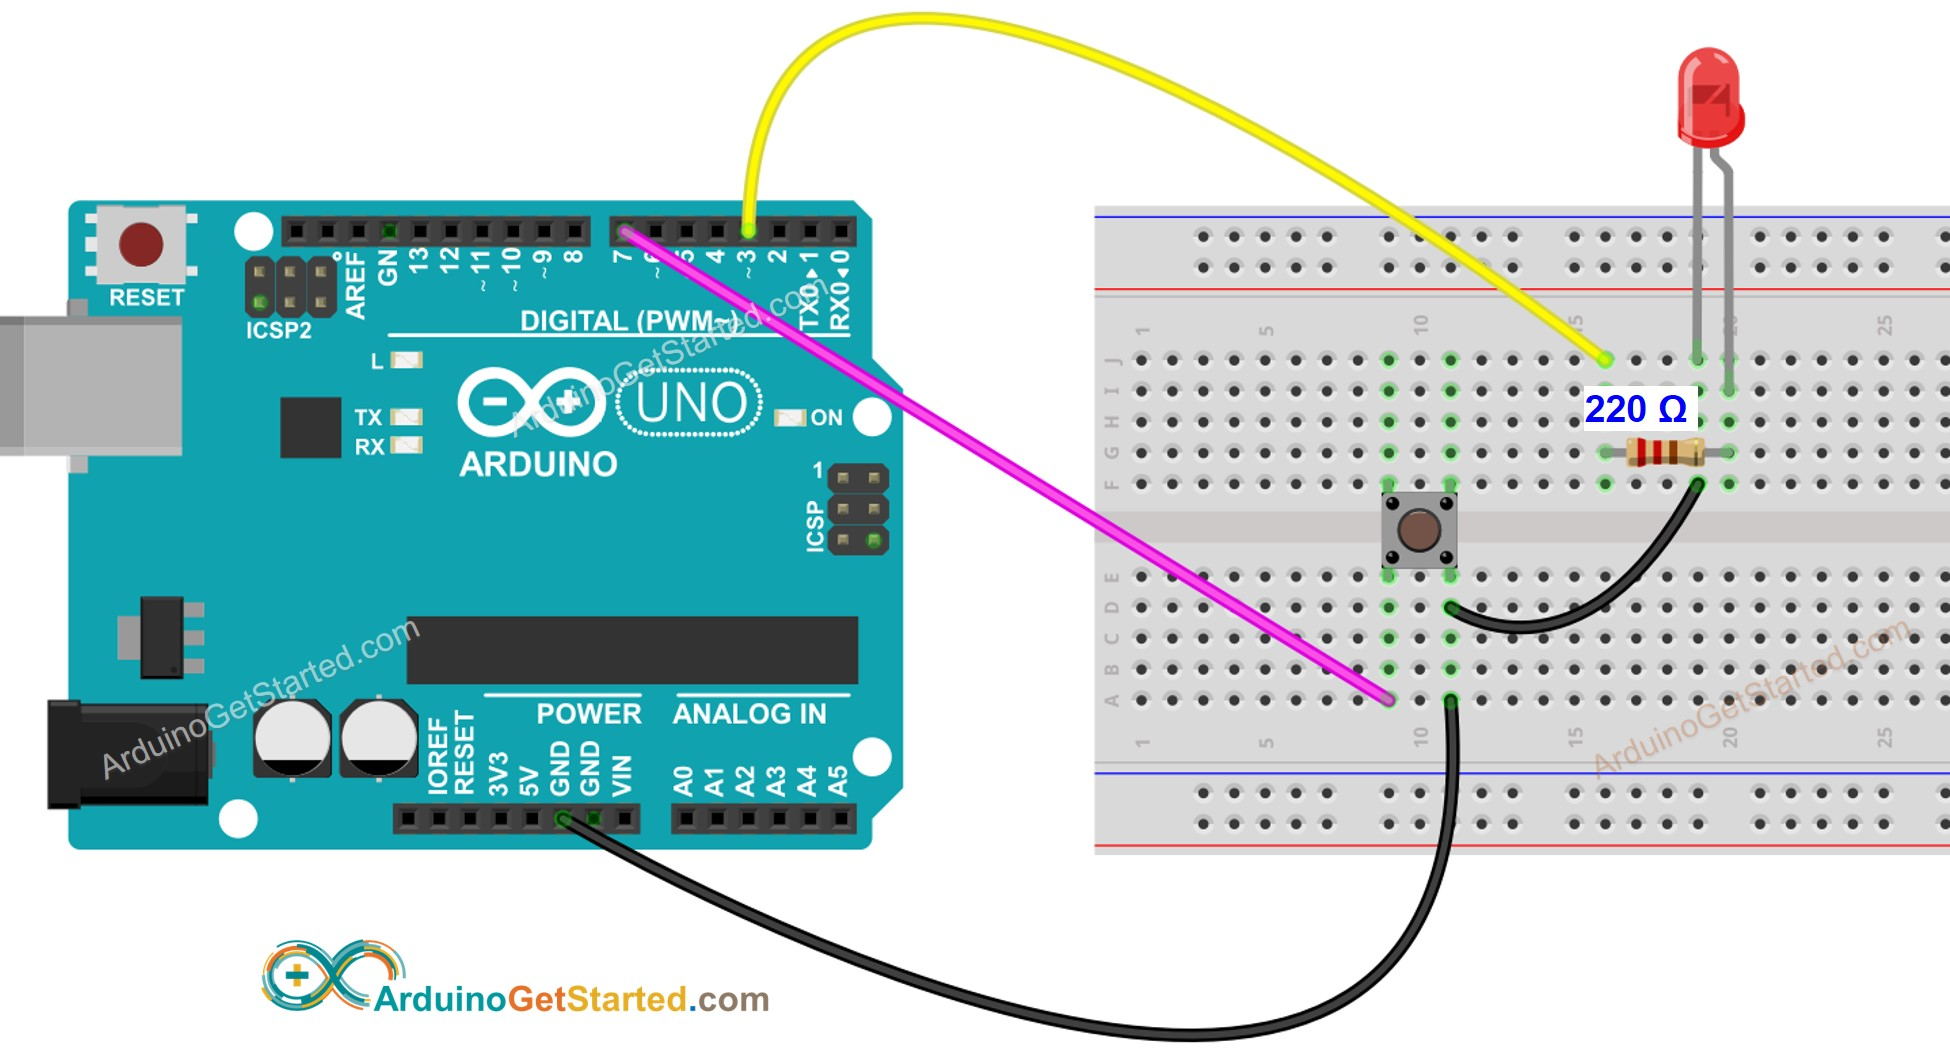
\includegraphics[width=\textwidth]{Pics/button-led-wiring-diagram.jpg}
%	\caption{Aufbau der Testschaltung, dargestellt durch ein Arduino-Hardware und einem Breadboard mit LED, einem 202 \Omega Widerstand und einem Taster.}
%	\label{fig:breadboard_wirinig}
%\end{figure}

Um die Funktionsweise der SPI- und DMA-Klassen zu überprüfen wurden ein Codeabschnitte implementiert: einer für einen Master, einer für einen Slave.
Die Pinkonfiguration war für beide die Gleiche.
Für jede Hardware wurde jeweils ein SPI-Objekt und ein DMA-Objekt erstellt.

Im Code wurde implementiert, dass der Master ein 'A' sendet und auf eine Antwort wartet, während der Slave ein 'O' sendet und eine Nachricht wartet.
Der Master-Code wurde auf ein STM32Nucleo-C031C6, der Slave-Code auf ein STM32Nucleo-G0B1RE geflasht. 
Die beiden MCUs wurden über die in der projct\_config.hpp definierte Gpio-Objekte mit einander verbunden.
An die einzelnen Pins wurden dann Klammern eines Oszilloskops angeschlossen um die Signale von Systemclock SCK, Master-Out-Slave-In MOSI, Master-In-Slave-Out MISO und NSS/CS Negative-Slave-Select bzw. Chip-Select zu beobachten. 

\subsection{Testergebnisse}
% CMakeLists, Build, Compile
Beginnend mit der Auswahl der Hardware durch die Kombination von Makefilekonfigurationen (stm32\_config.mk bzw. esp\_config.mk), CMakeLists-Struktur und Factory-Imlpementierung konnte Schritt für Schritt eine Struktur erarbeitet werden, die im weiteren Verlauf fehlerfrei funktioniert hat.
Bei unerwartetem Verhalten aber entsprechende Fehlermeldungen ausgeben konnte.
Im Fall von STM32 Hardware, da hiervon mehr zur Auswahl stand und diese auch hauptsächlich in der Praxis verwendet wird, hat auch der Wechsel zwischen unterschiedlichen Familien, STM32C0xx und STM32G0xx, über die stm32\_config.mk reibungslos funktioniert.
Der Einsatz von definierten Makros, wie beispielsweise \texttt{TARGET\_PLATFORM} \texttt{MCU\_FAMILY} oder \texttt{MCU\_SPECIFIC}, um in den CMakeLists.txt-Dateien die entsprechenden Bibliotheken auszuwählen, Dateien hinzuzufügen sowie Abschnitte freizuschalten, hat sich als vorteilhaft für die Erstellung eines automatisierten Kompilations- und Buildprozesses innerhalb der gesamten Struktur erwiesen.
Darüber hinaus hatte dies eine erfolgreiche Erstellung der Hardwareobjekte durch die Factory zur Folge.
Die wählt anhand der Makros erst die richtige Plattform und im weiteren Verlauf die spezifische Hardware aus.
% GPIO

Mit einem erstellten Programm, das die neuen Gpio-Objekte und deren Funktionen verwendet, und der aufgebauten Schaltung konnten das Lese und Schreib verhalten erfolgreich überprüft werden.
Bei Betätigung des Tasters sollte die LED eingeschaltet werden; bei erneuter Betätigung dementsprechend wieder ausgeschaltet werden.
Dieses Verhalten wurde erfolgreich umgesetzt.

% SPI
Um die
% Oszi-Bild , wie es aussehen sollte
\begin{figure}[H]
	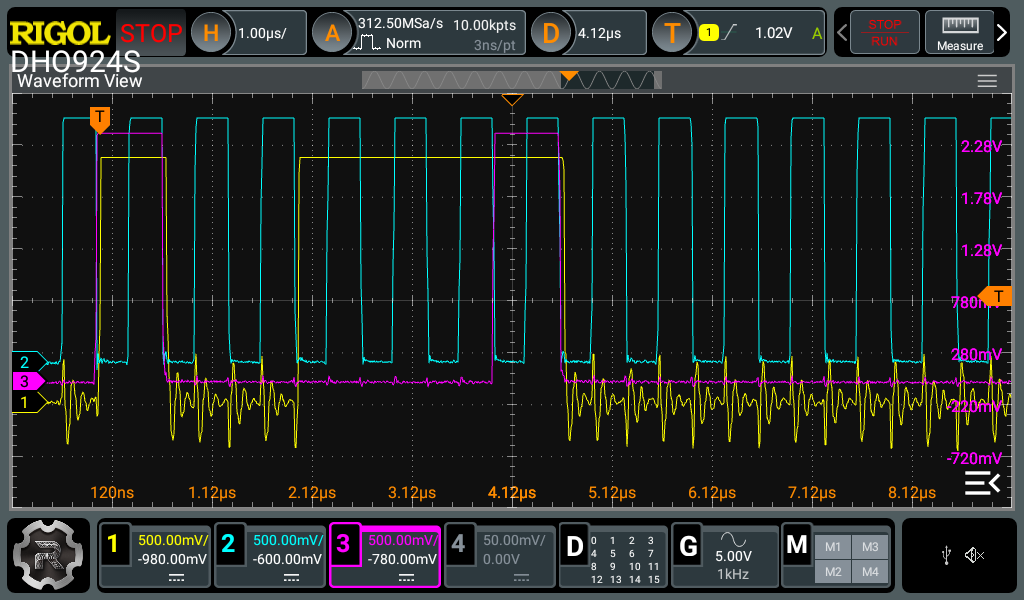
\includegraphics[width=\textwidth]{Pics/oszi_cube_spi_example.png}
	\caption{Screenshot des Osziloskopbildschirms. Dieser zeigt die Wellen für SCK (blau), MOSI (magenta) und MISO (gelb).}
	\label{fig:oszi_cube_spi_example}
\end{figure}

So sollten die Wellen auch mit dem Plattformunabhängigen Code aussehen.

\begin{figure}[H]
	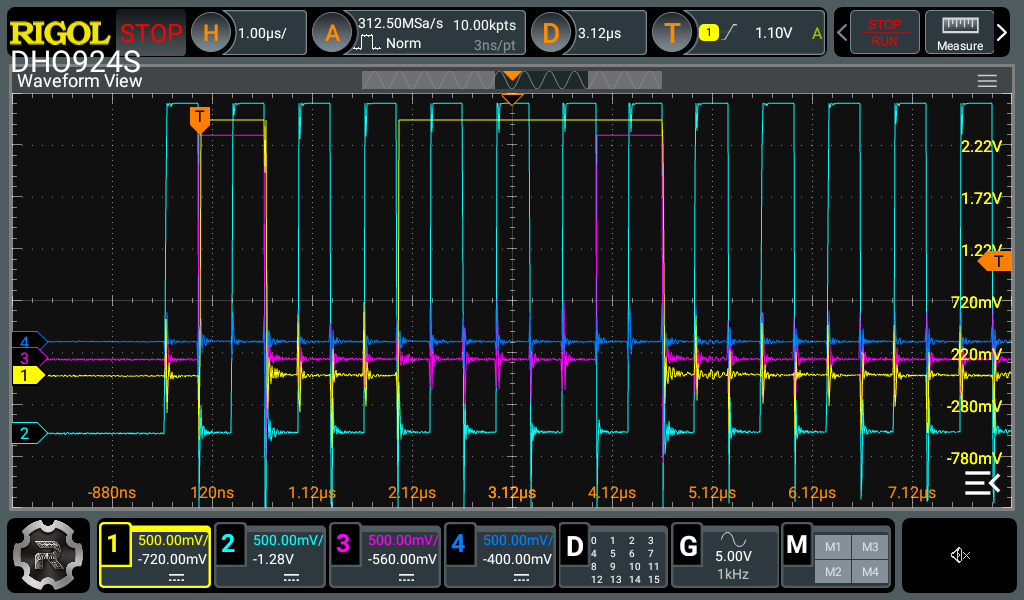
\includegraphics[width=\textwidth]{Pics/spi_signal_test.png}
	\caption{Screenshot einer erfolgreich SPI-Kommunikation, erstellt mit dem Code der HW\_API.}
\end{figure}


%Die Testumgebung umfasste sowohl das STM32C0-Board als auch ein ESP32-DevKit, jeweils verbunden mit Debug-Schnittstellen und notwendiger Peripherie.
%Die Tests wurden systematisch durchgeführt, indem jeder GPIO-Pin und jedes Peripheriemodul einzeln initialisiert, konfiguriert und gemessen wurde. 
%Für die SPI-Schnittstelle wurden verschiedene Kommunikationsszenarien simuliert, um mögliche Timing- oder Konfigurationsfehler zu erkennen.
%
%Die erzielten Ergebnisse zeigen, dass die HW\_API die spezifizierten Funktionen korrekt bereitstellt. 
%GPIO-Pins verhielten sich entsprechend der konfigurierten Pull-Up/Pull-Down-Einstellungen, und die SPI-Kommunikation konnte zuverlässig Daten übertragen. 
%Alle gemessenen Signalpegel lagen innerhalb der spezifizierten Grenzwerte der jeweiligen Plattformen. 
%Auffälligkeiten traten nicht auf, und die statische Analyse ergab keine kritischen Warnungen oder Verstöße gegen etablierte Embedded-Coding-Standards.
%
%Die Interpretation dieser Ergebnisse bestätigt die Robustheit und Portabilität der entwickelten Abstraktionsschicht. 
%Die modulare Struktur, die plattformspezifische Implementierungen sauber kapselt, erlaubt den Einsatz auf mehreren Mikrocontrollerfamilien, ohne dass Änderungen am Anwendungscode erforderlich sind. 
%Einschränkungen bestehen lediglich in der begrenzten Testabdeckung anderer STM32-Familien, die nicht direkt validiert wurden.

Zusammenfassend zeigt die Validierung, dass die HW\_API die geforderten funktionalen Anforderungen erfüllt, korrekt arbeitet und eine stabile Grundlage für die Implementierung plattformunabhängiger Embedded-Anwendungen darstellt. 
Die gewählten Testmethoden gewährleisten eine nachvollziehbare und reproduzierbare Überprüfung der Softwarequalität.

















































\listoffigures
\addcontentsline{toc}{chapter}{Abbildungsverzeichnis}
\listoftables
\addcontentsline{toc}{chapter}{Tabellenverzeichnis}
\lstlistoflistings
\addcontentsline{toc}{chapter}{Codeverzeichnis}
\addcontentsline{toc}{chapter}{Quellenverzeichnis}
\printbibliography

\end{document}